%\VignetteIndexEntry{Continuous time structural equation modelling with ctsem} 
%\VignetteKeyword{SEM, time series, panel data, dynamic models}
%\VignetteEngine{knitr::knitr} 
\documentclass[nojss]{jss}\usepackage[]{graphicx}\usepackage[]{color}
%% maxwidth is the original width if it is less than linewidth
%% otherwise use linewidth (to make sure the graphics do not exceed the margin)
\makeatletter
\def\maxwidth{ %
  \ifdim\Gin@nat@width>\linewidth
    \linewidth
  \else
    \Gin@nat@width
  \fi
}
\makeatother

\usepackage{Sweave}




%%%%%%%%%%%%%%%%%%%%%%%%%%%%%%
%% declarations for jss.cls %%%%%%%%%%%%%%%%%%%%%%%%%%%%%%%%%%%%%%%%%%
%%%%%%%%%%%%%%%%%%%%%%%%%%%%%%

%% almost as usual
\author{Charles C. Driver \\ Max Planck Institute for Human Development \And 
Johan H. L. Oud \\ Radboud University Nijmegen \AND
Manuel C. Voelkle \\ Humboldt University Berlin \\ Max Planck Institute for Human Development}
\title{Continuous Time Structural Equation Modelling With \proglang{R} Package \pkg{ctsem}}

%% for pretty printing and a nice hypersummary also set:
\Plainauthor{Charles C. Driver, Johan H. L. Oud, Manuel C. Voelkle} %% comma-separated
\Plaintitle{Continuous Time Structural Equation Modelling With R Package ctsem} %% without formatting
\Shorttitle{Continuous Time Structural Equation Modelling With \pkg{ctsem}} %% a short title (if necessary)

\Abstract{
Note: This paper introduces the frequentist, maximum likelihood based form of ctsem. For the Bayesian implementation, see \href{http://www.researchgate.net/publication/310747801_Hierarchical_Bayesian_Continuous_Time_Dynamic_Modeling}{Hierarchical Bayesian Continuous Time Dynamic Modelling} and \href{http://cran.r-project.org/web/packages/ctsem/vignettes/hierarchical.pdf}{Introduction to Hierarchical Continuous Time Dynamic Modelling With ctsem}. 

We introduce \pkg{ctsem} \citep{driver2017continuous}, an \proglang{R} package for continuous time structural equation modelling of panel (\textit{N} > 1) and time series (\textit{N} = 1) data using full information maximum likelihood. Most dynamic models (e.g., cross-lagged panel models) in the social and behavioural sciences are discrete time models. An assumption of discrete time models is that time intervals between measurements are equal, and that all subjects were assessed at the same intervals. Violations of this assumption are often ignored due to the difficulty of accounting for varying time intervals, therefore parameter estimates can be biased and the time course of effects becomes ambiguous. By using stochastic differential equations to estimate an underlying continuous process, continuous time models allow for any pattern of measurement occasions. By interfacing to \pkg{OpenMx}, \pkg{ctsem} combines the flexible specification of structural equation models with the enhanced data gathering opportunities and improved estimation of continuous time models. \pkg{ctsem} can estimate relationships over time for multiple latent processes, measured by multiple noisy indicators with varying time intervals between observations. Within and between effects are estimated simultaneously by modelling both observed covariates and unobserved heterogeneity. Exogenous shocks with different shapes, group differences, higher order diffusion effects and oscillating processes can all be simply modeled. We first introduce and define continuous time models, then show how to specify and estimate a range of continuous time models using \pkg{ctsem}.     
}

\Keywords{time series, longitudinal modelling, panel data, state space, structural equation modelling, continuous time, stochastic differential equation, dynamic models, Kalman filter, \proglang{R}}
\Plainkeywords{time series, longitudinal modelling, panel data, state space, structural equation modelling, continuous time, stochastic differential equation, dynamic models, Kalman filter, R} %% without formatting
%% at least one keyword must be supplied

%% publication information
%% NOTE: Typically, this can be left commented and will be filled out by the technical editor
%% \Volume{50}
%% \Issue{9}
%% \Month{June}
%% \Year{2012}
%% \Submitdate{2012-06-04}
%% \Acceptdate{2012-06-04}

%% The address of (at least) one author should be given
%% in the following format:
\Address{
Charles Driver\\
Center for Lifespan Psychology\\
Max Planck Institute for Human Development\\
Lentzeallee 94, 14195 Berlin\\
Telephone: +49 30 82406-367
E-mail: \email{driver@mpib-berlin.mpg.de}\\
URL: \url{http://www.mpib-berlin.mpg.de/en/staff/charles-driver}
}
%% It is also possible to add a telephone and fax number
%% before the e-mail in the following format:
%% Telephone: +43/512/507-7103
%% Fax: +43/512/507-2851

%% for those who use Sweave please include the following line (with % symbols):
%% need no \usepackage{Sweave.sty}

%% end of declarations %%%%%%%%%%%%%%%%%%%%%%%%%%%%%%%%%%%%%%%%%%%%%%%

\shortcites{boker2014openmx, boker2011openmx:, neale2015openmx, iacus2015pkgsde, king2010pkgpomp} %set any articles with more than 6 authors to short citation style first

\widowpenalty=50000
\clubpenalty=50000
\raggedbottom

\usepackage{amsmath} %for multiple line equations
\newcommand\numberthis{\addtocounter{equation}{1}\tag{\theequation}} %for adding numbers to specific lines

% Set lowercase greek letters to non-italicised

\usepackage[libertine]{newtxmath}
\usepackage[pdftex]{thumbpdf}
% \usepackage{amsfonts}
%\newcommand{\bmmax}{3}  
%\newcommand{\hmmax}{0}
%\usepackage[bm]

% \makeatletter
% \re@DeclareMathSymbol{\alpha}{\mathord}{lettersA}{11}
% \re@DeclareMathSymbol{\beta}{\mathord}{lettersA}{12}
% \re@DeclareMathSymbol{\gamma}{\mathord}{lettersA}{13}
% \re@DeclareMathSymbol{\delta}{\mathord}{lettersA}{14}
% \re@DeclareMathSymbol{\epsilon}{\mathord}{lettersA}{15}
% \re@DeclareMathSymbol{\zeta}{\mathord}{lettersA}{16}
% \re@DeclareMathSymbol{\eta}{\mathord}{lettersA}{17}
% \re@DeclareMathSymbol{\theta}{\mathord}{lettersA}{18}
% \re@DeclareMathSymbol{\iota}{\mathord}{lettersA}{19}
% \re@DeclareMathSymbol{\kappa}{\mathord}{lettersA}{20}
% \re@DeclareMathSymbol{\lambda}{\mathord}{lettersA}{21}
% \re@DeclareMathSymbol{\mu}{\mathord}{lettersA}{22}
% \re@DeclareMathSymbol{\nu}{\mathord}{lettersA}{23}
% \iftx@altnu
% \re@DeclareMathSymbol{\nu}{\mathord}{lettersA}{40}
% \fi
% \re@DeclareMathSymbol{\xi}{\mathord}{lettersA}{24}
% \re@DeclareMathSymbol{\pi}{\mathord}{lettersA}{25}
% \re@DeclareMathSymbol{\rho}{\mathord}{lettersA}{26}
% \re@DeclareMathSymbol{\sigma}{\mathord}{lettersA}{27}
% \re@DeclareMathSymbol{\tau}{\mathord}{lettersA}{28}
% \re@DeclareMathSymbol{\upsilon}{\mathord}{lettersA}{29}
% \re@DeclareMathSymbol{\phi}{\mathord}{lettersA}{30}
% \re@DeclareMathSymbol{\chi}{\mathord}{lettersA}{31}
% \re@DeclareMathSymbol{\psi}{\mathord}{lettersA}{32}
% \re@DeclareMathSymbol{\omega}{\mathord}{lettersA}{33}
% \re@DeclareMathSymbol{\varepsilon}{\mathord}{lettersA}{34}
% \re@DeclareMathSymbol{\vartheta}{\mathord}{lettersA}{35}
% \re@DeclareMathSymbol{\varpi}{\mathord}{lettersA}{36}
% \re@DeclareMathSymbol{\varrho}{\mathord}{lettersA}{37}
% \re@DeclareMathSymbol{\varsigma}{\mathord}{lettersA}{38}
% \re@DeclareMathSymbol{\varphi}{\mathord}{lettersA}{39}
% \makeatother
\IfFileExists{upquote.sty}{\usepackage{upquote}}{}
\begin{document}
%  \SweaveOpts{concordance = TRUE} %% I GUESS THIS COMMAND NEEDS TO GO SOMEWHERE ELSE 
%% include your article here, just as usual
%% Note that you should use the \pkg{}, \proglang{} and \code{} commands.


\newpage
\section[Introduction]{Introduction}\nopagebreak
Dynamic models, such as the well known vector autoregressive model, are widely used in the social and behavioural sciences. They allow us to see how fluctuations in processes relate to later values of those processes, the effect of an input at a particular time, how the various factors relate to average levels of the processes, and many other possibilities.
% are widely used in the social and behavioural sciences \citep{mcardle2009latent}. 
Some examples with panel data include the impact of European institutional changes on business cycles \citep{canova2012institutional}, the coupling between sensory and intellectual functioning \citep{ghisletta2005exploring}, or the analysis of bidirectional links between children's delinquency and the quality of parent-child relationships \citep{keijsers2011bidirectional}. 
% Dynamic models are not only used for the analysis of panel data, but are also common in the analysis of single subject time series data. 
Examples of single subject approaches are studies on the decline in pneumonia rates in the USA after a vaccine introduction \citep{grijalva2007decline}, or the lack of a relationship between antidepressant sales and public health in Iceland \citep{helgason2004antidepressants}. 
%% mv: make sure, are all of these are examples which would be better analyze in ct
% cd: I don't really like so many examples, feels like a lot of time spent for it if I find good continuous applications.
At present, applications of dynamic models in the social and behavioural sciences are almost exclusively limited to \textit{discrete time models}. In discrete time models it is generally assumed that time progresses in discrete steps, that time intervals between measurement occasions are equal, and that, in case of panel data, subjects are assessed with the same time intervals. In many cases, these assumptions are not met, resulting in biased parameter estimates and a misunderstanding of the strength and time course of effects. This concept is illustrated in Figure \ref{fig:discretecomparison} (with a comprehensive example in Appendix \ref{appendix:discretecomparison}). In the upper panel, Figure \ref{fig:discretecomparison} shows a true autoregressive effect of .80 between observed variables (represented by squares), assuming equal intervals of length $\Delta$\textit{t} = 1 (represented by equal distances between observed variables), while the lower panel shows a process with two intervals of $\Delta$\textit{t} = 1 and one interval $\Delta$\textit{t} = 2. In the top panel, the meaning of the estimate of .80 is clear -- it refers to the autoregression estimate for 1 unit of time. In the lower case, however, the autoregression estimate of .73 is ambiguous -- it is too low to characterise the relation between the first three occasions (correct value of .80 is in brackets) and too high between the last two occasions (correct value of .64). 

\begin{figure}[!h]
\centering
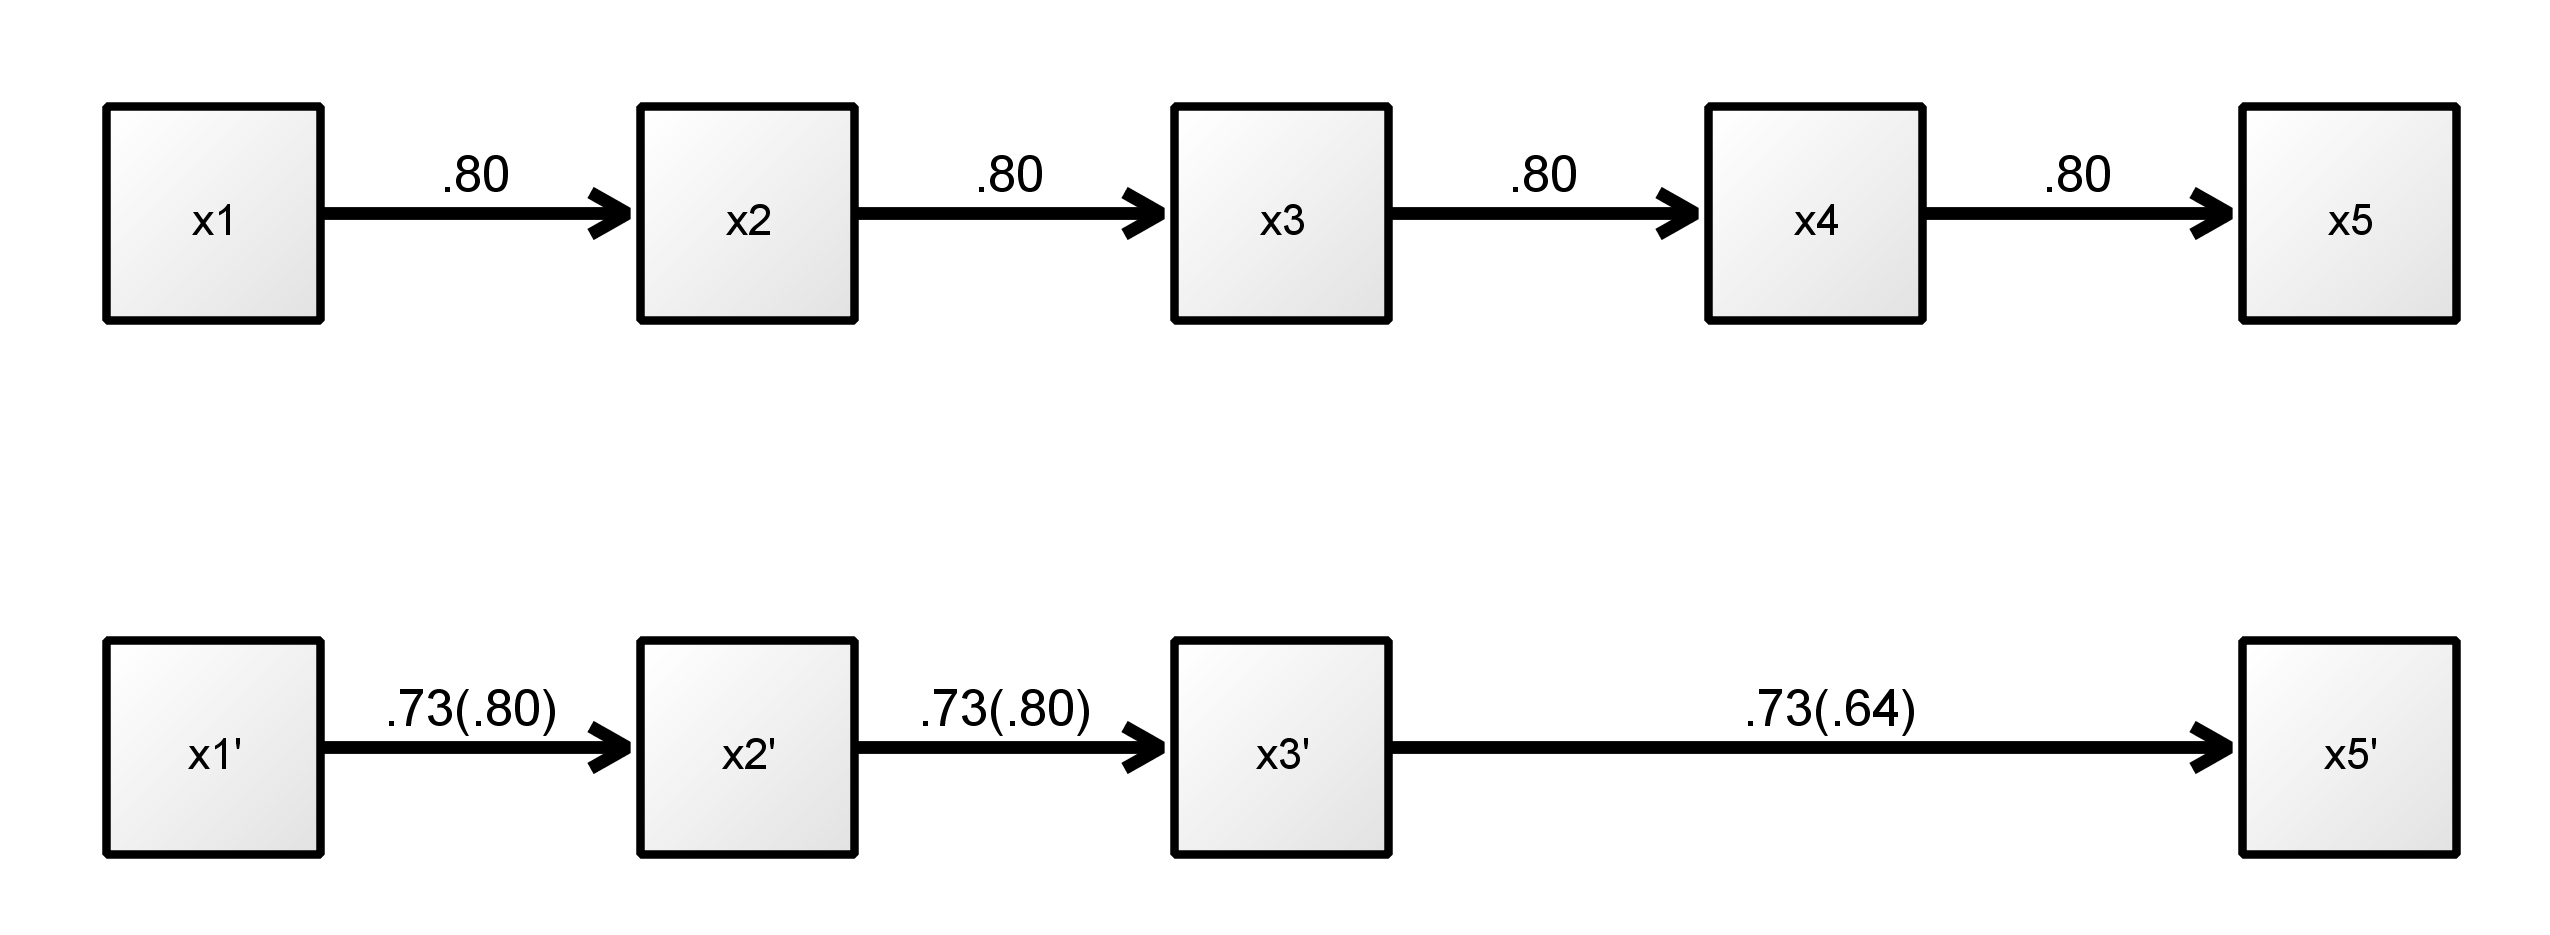
\includegraphics[]{pathdiagramdiscretecomparison}
\caption{ \label{fig:discretecomparison} Two autoregressive processes, each exhibiting a true autoregressive effect of .80 for 1 unit of time. The top process is measured with equal time intervals (represented by the space between observations) of 1 unit, while the lower process has unequal intervals.}
\end{figure}

Obviously, parameter estimates and, thus, scientific conclusions, are biased when observation intervals vary and this is not adequately accounted for. In simple cases, such as the example in Figure \ref{fig:discretecomparison}, additional variables -- so called phantom variables \citep{rindskopf1984using}, with missing values for all individuals -- could be added in order to artificially create equally spaced time intervals. For example, an additional variable could be specified at t4, resulting in equal time intervals and permitting the use of standard discrete time models. For complex patterns of individually varying time intervals, however, this approach quickly becomes untenable \citep{voelkle2013continuous}. Furthermore, with discrete time models it is difficult to compare results obtained from different studies with unequal time intervals, which poses a limitation to the production of cumulative knowledge in science \citep{voelkle2012sem}.

\textit{Continuous time models} overcome these problems, offering researchers the possibility to estimate parameters free from bias due to unequal intervals, easily compare between studies and datasets with different observation schedules, gather data with variable time intervals between observations, understand changes in observed effects over time, and parsimoniously specify complex dynamics. Although continuous time models have a long history \citep{coleman1964introduction, hannan1979methods}, their use in the social sciences is still uncommon. At least in part, this is due to a lack of suitable software to specify and estimate continuous time models. With the introduction of \pkg{ctsem} in this article, we want to overcome this limitation. Although we will define continuous time models in the next section and provide several examples in the sections thereafter, a comprehensive treatment of continuous time models is beyond the scope of this article. For a more general introduction to continuous time models by means of SEM, the reader is referred to \citet{voelkle2012sem}. For additional information on the technical details we refer the reader to \citet{oud2000continuous}. 

% The \proglang{R} package \pkg{ctsem} interfaces to \pkg{OpenMx} \citep{boker2011openmx:}, a powerful general purpose SEM and modelling package for \proglang{R} \citep{r_core_team2014r:}. This allows \pkg{ctsem} to capitalize on all the possibilities of structural equation models, including manifest and latent variables, flexibility in imposing parameter constraints, multiple group functionality, as well as the use of different fitting functions and non-linear constraints. Most importantly, by interfacing to \pkg{OpenMx} the user may tailor standard continuous time models to his or her specific needs. \pkg{OpenMx} was chosen as the basis for \pkg{ctsem} because of its capacity to incorporate the necessary matrix algebra constraints, such as the matrix exponential.

While there are already a range of packages that deal with continuous time (stochastic differential equation) models in \proglang{R}, most focus on single subject applications. These include \pkg{sde} \citep{iacus2015pkgsde}, \pkg{yuima} \citep{brouste2014pkgyuima}, \pkg{SIM.DiffProc} \citep{boukhetala2014pkgsim}, \pkg{cts} \citep{wang2013pkgcts}, \pkg{POMP} \citep{king2010pkgpomp}. For multi-subject approaches, \pkg{OpenMx} \citep{neale2015openmx} now includes the function \code{mxExpectationStateSpaceContinuousTime}, which can be combined with the function \code{mxFitFunctionMultigroup} for fixed effects based group analysis.  \pkg{ctsem} is focused on providing an accessible workflow, for full information maximum likelihood estimation of continuous time multivariate autoregressive models with random intercepts,  for both time series and panel data. Using \pkg{ctsem}, one may specify: Cross lagged panel models; latent growth curve models; random intercepts at the latent or manifest level; damped oscillators; dynamic factor analysis models; constant or time dependent exogenous predictors; continuous time ARMAX models from the time series tradition; multiple groups or individuals with different parameters; or any combination of the preceding. First order models should be generally equivalent to discrete time first order models, if there is no variability in time intervals. For an example of this equivalence in regards to dual change score models see \citet{voelkle2015relating}. For an \proglang{R} script and plot comparing estimates of a simple autoregressive model using \pkg{ctsem} and other packages, see Appendix \ref{app:appendixA}.

% There already exist a number of packages that can perform for stochastic calculus in \proglang{R}; see \CRANpkg{sde}~\citep{Stefano2009} and \CRANpkg{yuima} project package for SDEs~\citep{Stefano2014} a freely available on CRAN, this packages provides functions for simulation and inference for stochastic differential equations. It is the accompanying package to the book of~\citet{Stefano2008}.

The remainder of this article is organised as follows: in Section \ref{sec:formalspec}, we provide a formal definition of the continuous time models dealt with in this package. In Section \ref{sec:ctsemoverview} we will show how to install \pkg{ctsem} and give an overview of the package. In Section \ref{sec:datastructure}, we will review different data structures and discuss the role of time in continuous time models. In Section \ref{sec:modelspec}, we will show how to specify continuous time models in \pkg{ctsem}, followed by a discussion of model estimation and testing in Section \ref{sec:modelfit}. In Section \ref{sec:extensions} we will discuss various extensions of basic continuous time models, including unobserved heterogeneity, time dependent and time independent exogenous predictors, time series, multiple group models, higher order, and oscillating models. We will end with some discussion of various specification options and tips for model fitting in Section \ref{sec:tips}, and point to current limitations and future research and development directions in Section \ref{sec:limitations}.

\section{Continuous time models: fundamentals}\label{sec:formalspec}\nopagebreak
The class of continuous time models implemented in \pkg{ctsem} is represented by the multivariate stochastic differential equation:

\begin{equation}
\label{eq:process1}
\mathrm{  d \boldsymbol{\eta}_{\mathnormal{i}} \mathnormal{(t)} =
\bigg( \textbf{A} \boldsymbol{\eta}_{\mathnormal{i}} ( \mathnormal{t} ) +
\boldsymbol{\xi}_{\mathnormal{i}} +
\mathbf{Bz}_{\mathnormal{i}} +
\mathbf{M}\boldsymbol{\chi}_{\mathnormal{i}} ( \mathnormal{t} )  \bigg) d \mathnormal{t} +
\textbf{G} d \textbf{W}_{\mathnormal{i}}(\mathnormal{t})  }
\end{equation}


Vector $\boldsymbol{\eta}_{\mathnormal{i}}(\mathnormal{t})\in\mathbb{R}^{v}$ is a \textit{v}-variable vector of the processes of interest at time $\mathnormal{t}$, for subject $\mathnormal{i}$. The matrix $\textbf{A}\in \mathbb{R}^{v \times v}$ represents the so-called drift matrix, with auto effects on the diagonal and cross effects on the off-diagonals characterising the temporal relationships of the processes. 

The long term  level of processes $\boldsymbol{\eta}_{\mathnormal{i}}(\mathnormal{t})$ is determined by the \textit{v}-length vector of random variables $\boldsymbol{\xi}_{\mathnormal{i}}$, with $\boldsymbol{\xi}_{\mathnormal{i}}\sim \mathrm{N}(\boldsymbol{\kappa}, \boldsymbol{\phi_{\xi}}) \textnormal{ for every } \textit{i}$, where vector $\boldsymbol{\kappa}\in \mathbb{R}^{v}$ denotes the continuous time intercepts, and matrix $\boldsymbol{\phi_{\xi}}\in \mathbb{R}^{v \times v}$ the covariance across subjects. $\boldsymbol{\xi}_{\mathnormal{i}}$ sets the long-term level of the processes and the long-term differences between the processes of individual subjects -- without it the processes of a stable model would all trend towards zero in the long-run.

The matrix $\textbf{B}\in \mathbb{R}^{v \times p}$ represents the effect of the $p$-length vector of (fixed) time independent predictors $\textbf{z}\in\mathbb{R}^{p}$ on processes $\boldsymbol{\eta}_{\mathnormal{i}}(\mathnormal{t})$. Time independent predictors would typically be variables that differs between subjects, but are constant within subjects for the time range in question.

Time dependent predictors $\boldsymbol{\chi}_i(t)$ represent inputs to the system that vary over time and are independent of fluctuations in the system. Equation \ref{eq:process1} shows a generalised form for time dependent predictors, that could be treated a variety of ways dependent on the assumed time course (or shape) of time dependent predictors. We use a simple impulse form, in which the predictors are treated as impacting the processes only at the instant of an observation. When necessary, the evolution over time can be modeled by extending the state matrices. This is demonstrated in the level change example in Section \ref{sec:tdpreds}, wherein a model containing only the basic impulse has a persistent level change effect added. To achieve the impulse form we replace part of Equation \ref{eq:process1} as follows:

\begin{equation}
\label{eq:spike}
\mathrm{\boldsymbol{\chi}_{\mathnormal{i}} ( \mathnormal{t} ) =\sum_{\mathnormal{u} \in \mathnormal{U_i}}  \mathbf{x}_{\mathnormal{i,u}} \boldsymbol{\delta} ( \mathnormal{t-u} )     }
\end{equation}

Here, time dependent predictors $\mathbf{x}_{i,u} \in \mathbb{R}^{l}$ are observed at times $u \in U_i \subset \mathbb{R}$. The Dirac delta function $\boldsymbol{\delta}(t-u)$ is a generalised function that is $\infty$ at 0 and 0 elsewhere, yet has an integral of 1 (when 0 is in the range of integration). It is useful to model an impulse to a system, and here is scaled by the vector of time dependent predictors $\mathbf{x}_{i,u}$.  The effect of these impulses on processes $\boldsymbol{\eta}_{\mathnormal{i}}(\mathnormal{t})$ is then $\textbf{M}\in \mathbb{R}^{v \times l}$.

$\textbf{W}_{\mathnormal{i}}(\mathnormal{t}) \in \mathbb{R}^{v}$ represent independent Wiener processes, with a Wiener process being a random-walk in continuous time. $\textnormal{d}\textbf{W}_{\mathnormal{i}}(\mathnormal{t})$ is meaningful in the context of stochastic differential equations, and represents the stochastic error term, an infinitesimally
small increment of the Wiener process. Lower triangular matrix $\mathbf{G}\in \mathbb{R}^{v \times v}$ represents the effect of this noise on the change in $\boldsymbol{\eta}_{\mathnormal{i}}(\mathnormal{t})$.  \textbf{Q}, where $\textbf{Q} = \textbf{GG}^\top $, represents the variance-covariance matrix of the diffusion process in continuous time.

The solution of the stochastic differential Equation \ref{eq:process1} for any time interval $t-t_0$, with $t > t_0$ is:


\begin{align*}
\boldsymbol{\eta}_{\mathnormal{i}}(\textit{t}) = \: &
\mathrm{e}^{ \textbf{A} (\mathnormal{t-t_0})  }  \boldsymbol{\eta}_{\mathnormal{i}}(\mathnormal{t_0}) \: + \\
&\textbf{A}^{-1} [\mathrm{e}^{\textbf{A} \mathnormal{(t-t_0)} } - \textbf{I}] \boldsymbol{\xi}_{\mathnormal{i}} \: + \\
&\textbf{A}^{-1} [\mathrm{e}^{\textbf{A} \mathnormal{(t-t_0)} } - \textbf{I}]\textbf{Bz}_{\mathnormal{i}} \: + \\
&\mathbf{M} \mathrm{ \sum_{\mathnormal{u} \in \mathnormal{U_i}}  \mathbf{x}_{\mathnormal{i,u}} \boldsymbol{\delta} ( \mathnormal{t-u} )} \: + \\
&\int_{\mathnormal{t_0}}^\mathnormal{t} \mathrm{e}^{\textbf{A} \mathnormal{(t-s)} } \textbf{G}\textrm{d}\textbf{W}_{\mathnormal{i}}\mathnormal{(s)} \numberthis 
\label{eq:solution}
\end{align*}

The five summands of this equation correspond to the five of Equation \ref{eq:process1}, and give the
link between the continuous time model and discrete instantiations of the process. 

The last summand of Equation \ref{eq:solution}, the integral of the diffusion over the given time interval, exhibits covariance matrix:

\begin{equation}
\label{eq:dyncov}
\mathrm{cov \Big[ \int_{\mathnormal{t_0}}^\mathnormal{t} \mathrm{e}^{\textbf{A}(\mathnormal{t-s})} \textbf{G}d\textbf{W}_{\mathnormal{i}}(\mathnormal{s})\Big] \: 
= \: \mathnormal{\int_{t_0}^t } \mathrm{e}^{\textbf{A} \mathnormal{(t-s)} }\textbf{Q} \mathrm{e}^{\textbf{A}^\top \mathnormal{(t-s)}} d\mathnormal{s} \: 
= \: irow \big( \textbf{A}_{\#}^{-1} [\mathrm{e}^{\textbf{A}_{\#} \mathnormal{(t-t_0)} } - \textbf{I}] \: row (\textbf{Q}) \big) }
\end{equation}

Where $\textbf{A}_{\#} = \textbf{A} \otimes \textbf{I} + \textbf{I} \otimes \textbf{A} $, with $\otimes$ denoting the Kronecker-product, row is an operation that takes elements of a matrix rowwise and puts them in a column vector, and irow is the inverse of the row operation.

The process vector $\boldsymbol{\eta}_{\mathnormal{i}}(\mathnormal{t})$ may be directly observed or latent with measurement model

\begin{equation}
\label{eq:measurement}
\mathrm{\textbf{y}_{\mathnormal{i}} \mathnormal{(t)} = \boldsymbol{\Gamma}_{\mathnormal{i}} + \boldsymbol{\Lambda} \boldsymbol{\eta}_{\mathnormal{i}} ( \mathnormal{t} ) + \boldsymbol{\zeta}_{\mathnormal{i}}\mathnormal{(t)},  
\quad \text{where } \boldsymbol{\zeta}\mathnormal{(t)} \sim  \mathrm{N} ( \textbf{0} , \boldsymbol{\Theta} ) ,
\quad \text{and } \boldsymbol{\Gamma} \sim  \mathrm{N} ( \boldsymbol{\tau} , \Psi ) }
\end{equation}

where \textit{c}-length vector $\boldsymbol{\tau}$ is the expected value of $\boldsymbol{\Gamma}_{\mathnormal{i}}$, which is distributed across subjects according to covariance matrix $\boldsymbol{\Psi} \in \mathbb{R}^{\mathnormal{c \times c}}$ (referred to later as \textit{manifest traits} -- see Section \ref{sec:heterogeneity}). $\boldsymbol{\Lambda} \in \mathbb{R}^{c \times v}$ is a matrix of factor loadings, $\textbf{y}_{\mathnormal{i}} (\mathnormal{t})\in\mathbb{R}^{c}$ is a vector of manifest variables, and residual vector $\boldsymbol{\zeta}_i \in \mathbb{R}^{c}$ has covariance matrix $\boldsymbol{\Theta} \in\mathbb{R}^{c \times c}$.

\subsection{Continuous time and SEM}\nopagebreak
Continuous time models have already been implemented as structural equation models, using either non-linear algebraic constraints \citep{oud2000continuous} or linear approximations of the matrix exponential \citep{oud2002continuous}. Our formulation uses either the SEM RAM (reticular action model) specification as per \citet{mcardle1984algebraic}, or the state space form recently added to \pkg{OpenMx} \citep{neale2015openmx, hunter2014state}. For details on the equivalence and differences between SEM and state space modelling techniques, see \citet{chow2010equivalence}. \pkg{ctsem} translates user specified input matrices and switches into an \pkg{OpenMx} model consisting of continuous time parameter matrices, algebraic transformations of these matrices to aid optimization (See Section \ref{sec:modelfit}), and algebraic transforms from the continuous time parameters to discrete time parameters for every unique time interval. Expectation matrices are then generated for each individual according to the specified inputs, constraints, and observed timing data. Optimization using either the Kalman filter or row-wise full information maximum likelihood (FIML) within \pkg{OpenMx} is used to estimate the parameters, typically with a first pass using a penalty term (or prior) to find a region of high probability without extreme parameters, and then a second FIML pass using the first as starting values.

To see exactly how the various matrices are transformed into a RAM SEM, one may run the following code after \pkg{ctsem} is installed (See Section \ref{sec:ctsemoverview}). This example comprises two latent processes, three observed indicators, a time dependent predictor, and two time independent predictors, across three time points of observation.

\begin{Schunk}
\begin{Sinput}
data('datastructure')
datastructure
semModel<-ctModel(n.latent=2, n.manifest=3, TRAITVAR='auto', 
  n.TIpred=2, n.TDpred=1, Tpoints=3, 
  LAMBDA=matrix(c(1,'lambda21', 0, 0,1,0),nrow=3))
semFit<-ctFit(datastructure, semModel, nofit=TRUE)
semFit$mxobj$A$labels
semFit$mxobj$S$labels
semFit$mxobj$M$labels
semFit$mxobj$F$values
\end{Sinput}
\end{Schunk}

% 
% , by minimising the minus two log likelihood, which is as follows: 
% 
% \begin{equation}
% \label{eq:fiml}
% \mathrm{
% \mathnormal{-2LL = \sum_{i = 1}^\textit{N}} \mathrm{log (2\pi) \textbf{V}}\mathnormal{_i} +
% log | \boldsymbol{\Sigma}_{\mathnormal{i}} | + 
% (\textbf{y}_{\mathnormal{i}} - \textbf{M}_{\mathnormal{i}})
% \boldsymbol{\Sigma}_{\mathnormal{i}}^{-1}
% (\textbf{y}_{\mathnormal{i}} - \textbf{M}_{\mathnormal{i}})^\top
% }
% \end{equation}
% 
% Where $\boldsymbol{\Sigma}_i$ is the filtered expected covariance matrix of individual \textit{i}, $\textbf{V}_i$ is the number of non-missing variables observed for that individual, and $\textbf{M}_i$ the model implied means vector for individual \textit{i}. 
% 
For more detailed information on the specification of continuous time structural equation models, the reader is referred to \citet{oud2000continuous, arnold1974stochastic, singer1998continuous, voelkle2012sem}. Note that while earlier incarnations of continuous time modelling focused on approaches to implement the matrix exponential, \pkg{OpenMx} now includes a form of the exponential recommended in computational contexts, the scaling and squaring approach with Pade approximation \citep{higham2009scaling}, which has been implemented in \pkg{ctsem} accordingly.

\section[ctsem package overview and installation]{\pkg{ctsem} package overview and installation} \label{sec:ctsemoverview}\nopagebreak
As \pkg{ctsem} is an \proglang{R} package, it requires \proglang{R} to be installed, available from \url{www.r-project.org} \citep{rcoreteam2014r}. 
The \proglang{R} package \pkg{OpenMx} \citep{neale2015openmx} is required, and although it will be installed automatically via CRAN if necessary, it is recommended to download it from \url{http://openmx.psyc.virginia.edu/}, to allow use of the NPSOL optimizer. 
\pkg{ctsem} is available via CRAN, so to install and load  within \proglang{R} simply use:

\begin{Schunk}
\begin{Sinput}
install.packages("ctsem")
library("ctsem")
\end{Sinput}
\end{Schunk}

For the latest development versions, \url{http://github.com/cdriveraus/ctsem} provides the Github repository, which can also be used to flag any issues noted or request support.

Estimating continuous time models via \pkg{ctsem} comprises four steps: First, the data must be adequately prepared (Section \ref{sec:datastructure}). Then, the continuous time model must be specified by creating a \pkg{ctsem} model object using the function \code{ctModel} (Sections \ref{sec:modelspec} and \ref{sec:extensions}). After specification, the model must be fit to the data using the function \code{ctFit}, after which \code{summary} and \code{plot} methods may be used to examine parameter estimates, standard errors, and fit statistics (Section \ref{sec:modelfit}). We will discuss these steps in the following.  

\section{Data structure} \label{sec:datastructure}\nopagebreak
Both a wide format (with time intervals) and a long format (with absolute times) are, as of version 2.5.0, available as input formats for ctsem. Wide format is the default, though \code{dataform='long'} can be specified in the arguments to the \code{ctFit} function. In general, a long format may be easier to work with, though a wide format may match existing panel data configurations in some cases. Conversion from long format with absolute times to wide format with is possible via the \code{ctLongToWide} and \code{ctIntervalise} functions, and conversion from wide to long is possible using the \code{ctWideToLong} and \code{ctDeintervalise} functions. The choice of time scale and treatment of the initial time point can influence results and will be discussed in Section \ref{sec:datatimescale}, though first time users may find it easier to return to later.

\subsection{Wide format} \label{sec:datawide}\nopagebreak 
The example data below depicts two individuals, observed at three occasions, on three manifest variables, one time dependent predictor, and two time independent predictors. A corresponding path diagram of one possible model for this data is shown in Figure \ref{fig:pathdiagramtwoprocessfull}. The data are ordered into blocks as follows: Manifest process variables, time dependent predictors, time intervals, time independent predictors. Manifest variables are grouped by \textit{measurement occasion} and ordered within this by \textit{variable}. In the example there are three manifest variables (Y1, Y2, Y3) assessed across three measurement occasions. In this case, the first three columns of the data (Y1\_T0, Y2\_T0, Y3\_T0) represent the three manifest variables at the first measurement occasion, time point 0, followed by the columns of the second measurement occasion and so on. Note that measurement occasions subsequent to the first may occur at different times for different individuals.  Also note the naming convention, wherein the variable name is followed by an underscore and T, followed by an integer denoting the measurement occasion, beginning at T0.  After the manifest variables, any time dependent predictors (there need not be any) are also grouped by \textit{measurement occasion} and ordered within this by \textit{variable} (changed since v2.2.0). These are named in the same way as the manifest variables, with the predictor name preceded by an underscore and T, then the measurement occasion integer beginning from 0. In the data below and the model in Figure \ref{fig:pathdiagramtwoprocessfull}, there is only one time dependent predictor, TD1, though more could be added. After the time dependent predictors, \textit{T}-1 time intervals are specified in chronological order, with column names dT followed by the number of the measurement occasion occurring \textit{after} the interval . That is, dT1 refers to the time interval between the first measurement occasion, T0, and the second, T1.  In continuous time modelling it is imperative to know the time point at which an observation takes place. Thus, while missing values on observed scores are no problem, missing values on time intervals are not allowed. Finally, two time independent predictors (TI1, TI2 -- the naming here is only with variable names) are contained in the last two columns of the data structure.

\begin {scriptsize}
\begin{Schunk}
\begin{Soutput}
  Y1_T0 Y2_T0 Y3_T0 Y1_T1 Y2_T1 Y3_T1 Y1_T2 Y2_T2 Y3_T2 TD1_T0 TD1_T1 TD1_T2  dT1   dT2  TI1   TI2
1  0.44 -0.83 -0.17  1.13 -2.44  0.31    NA    NA    NA  -1.67   0.15     NA 0.65 0.001 0.06 -2.05
2    NA  6.84  9.22  8.24  9.04  7.88  6.45  8.39  7.16   0.81  -1.97   -1.6 2.56 2.260 2.22 -1.41
\end{Soutput}
\end{Schunk}
\end{scriptsize}

\begin{figure}[p]
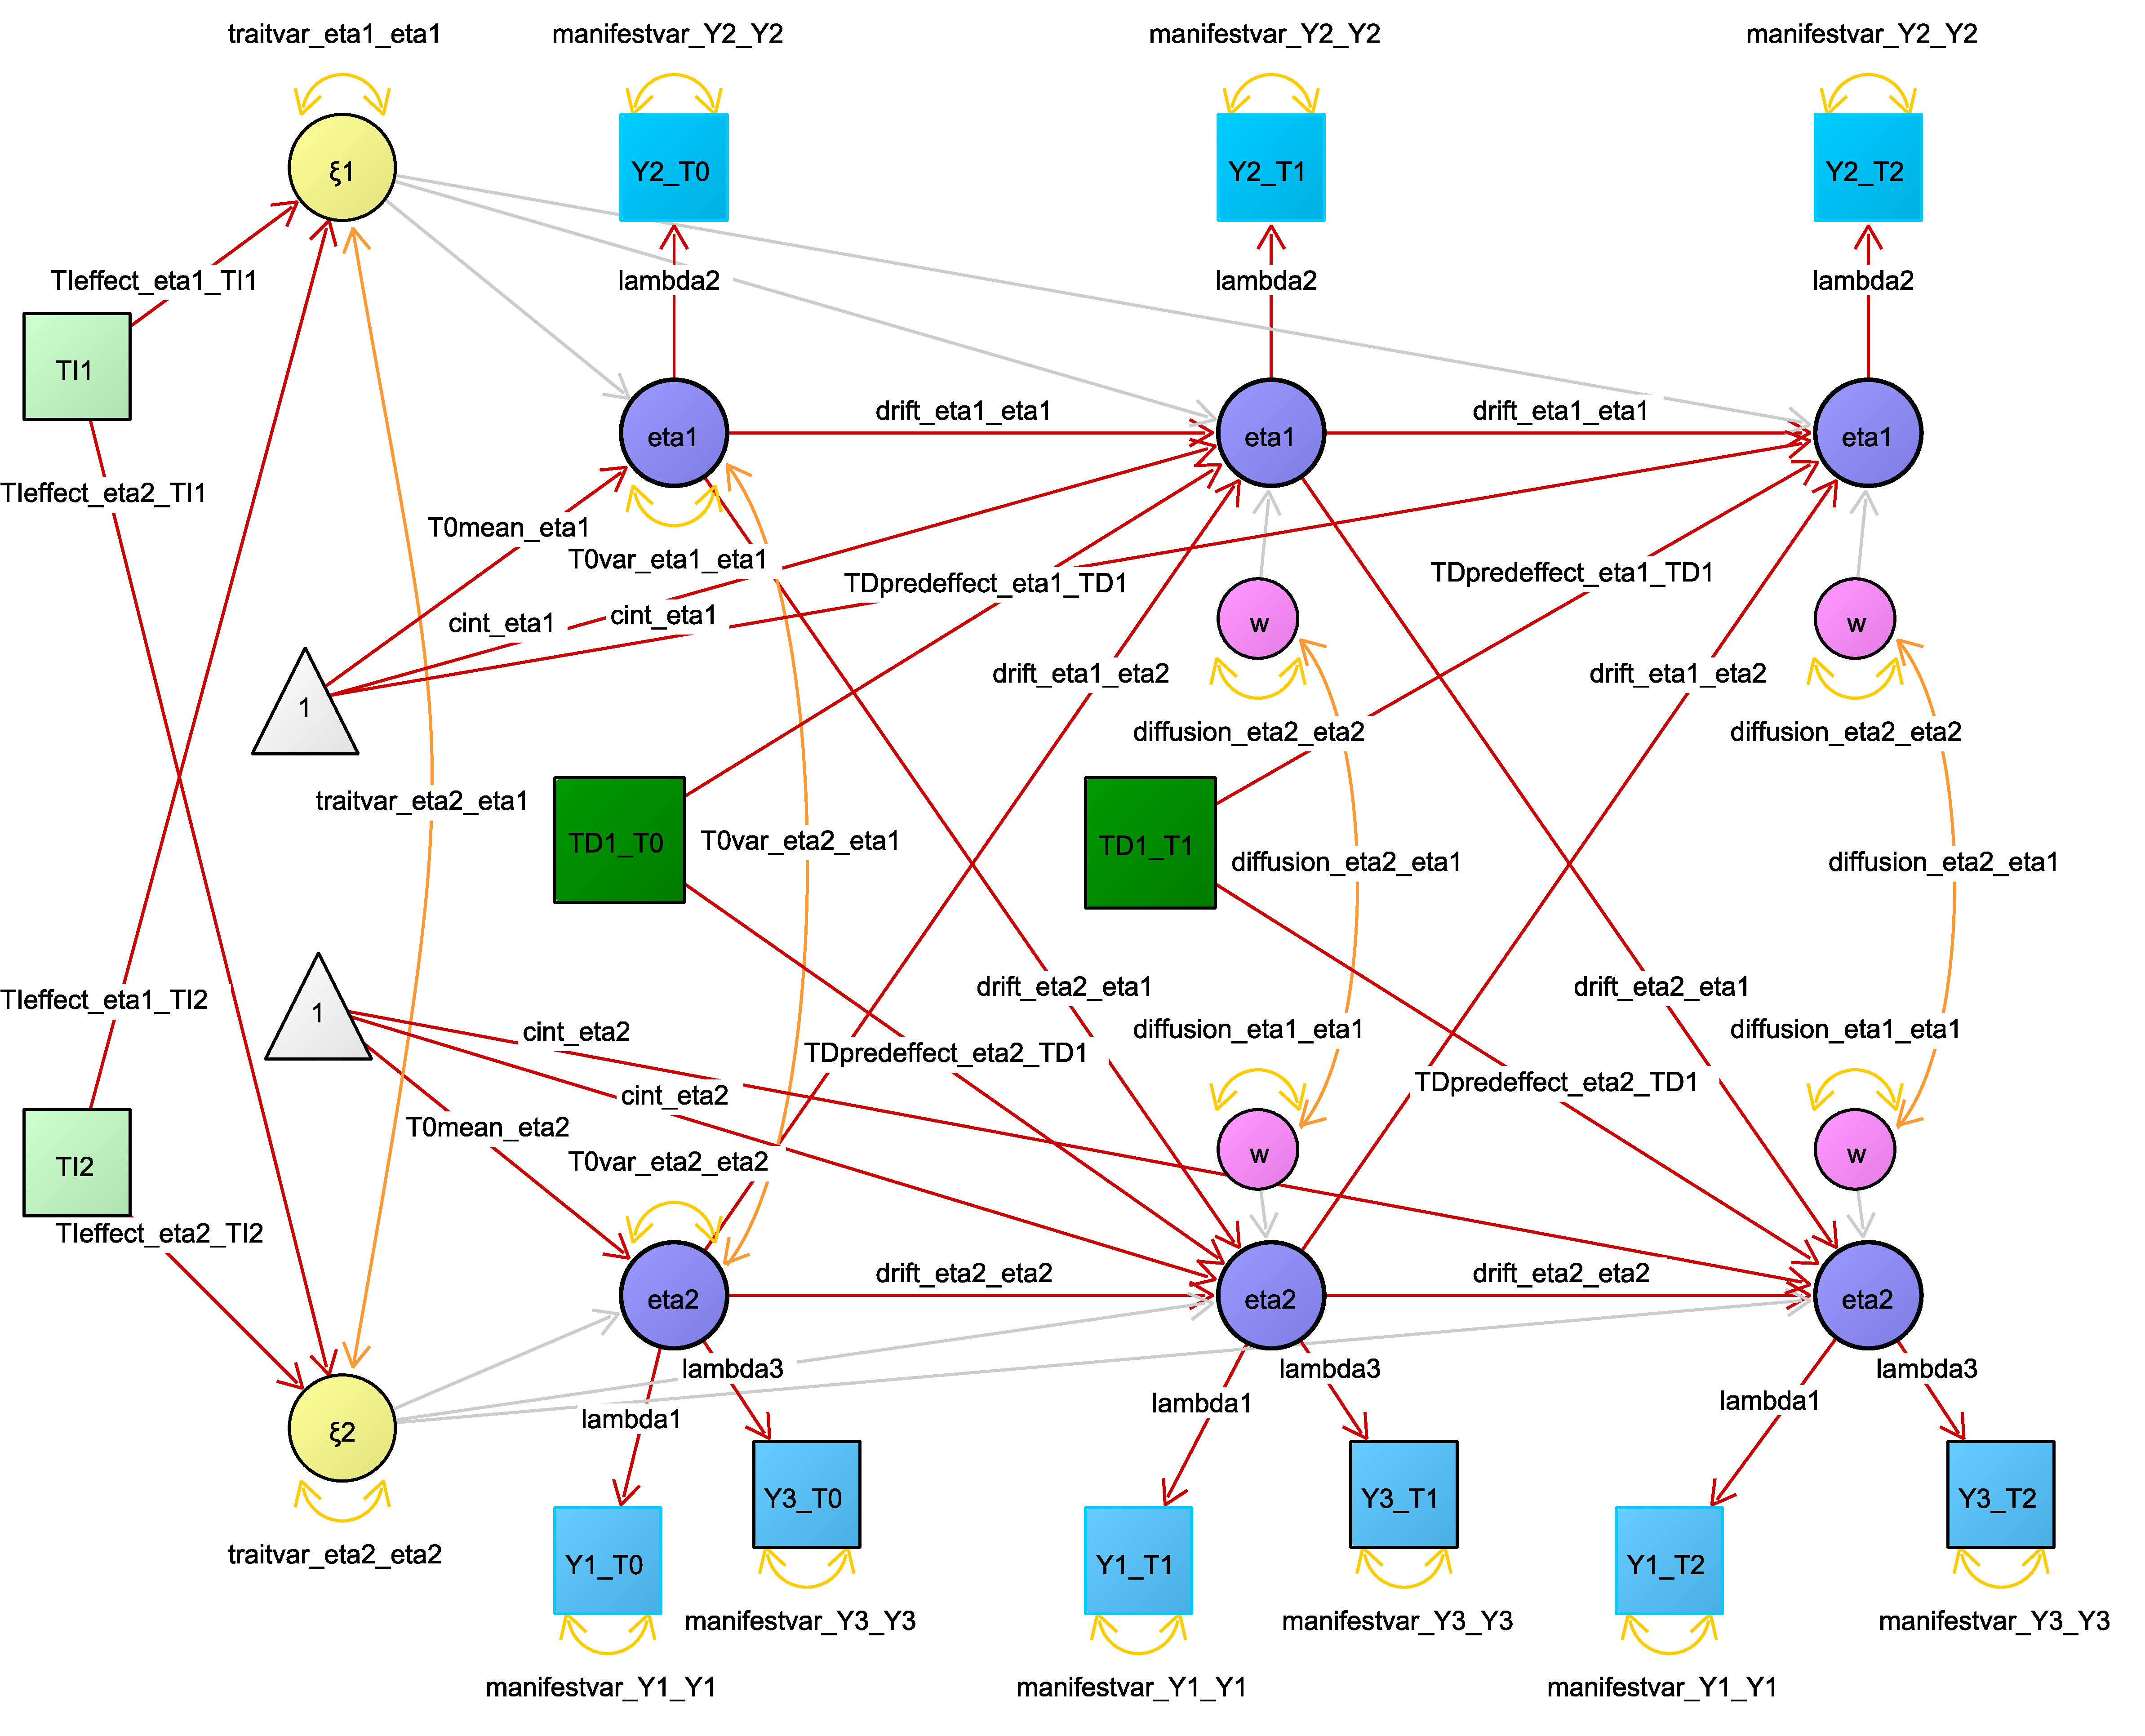
\includegraphics[width = \textwidth]{pathdiagramtwoprocessfull2}
\caption{ \label{fig:pathdiagramtwoprocessfull} The first three time points of a two process continuous time model, with three manifest indicators (blue) measuring 2 latent processes (purple), one time dependent predictor(dark green), and two time independent predictors (light green). Variance / covariance paths are in orange, regressions in red. Light grey paths indicate those that are constrained to a function of other parameters. Note that the value of parameters for all paths to latents at time 2 and higher do not directly represent the effect, rather, the effect depends on a function including the shown parameter and the time interval $\Delta$\textit{t}. Manifest intercepts are not shown.}
\end{figure}

\subsection{Long format with absolute times} \label{sec:datalong}\nopagebreak 
For the from long format, the data must contain a subject identification column, columns for every observed variable, and a time variable. Unlike for the wide format data, at this point additional unused variables in the long structure are no problem. In the example below, three manifest variables of interest (Y1, Y2, Y3) have been observed across a number of occasions, along with one time dependent predictor (TD1) and two time independent predictors (TI1, TI2). The variable 'time' contains the time when the measurement took place (e.g., in weeks from the beginning of the study). 

\begin{Schunk}
\begin{Soutput}
     id time    Y1    Y2    Y3   TD1   TI1   TI2
[1,]  1 0.00  5.37  6.05  7.35  2.77 -0.45 -0.23
[2,]  1   NA  5.90  3.58  7.19  1.15    NA -0.23
[3,]  1 0.89  5.92  5.05  5.09  1.55 -0.45 -0.23
[4,]  2 1.13    NA 10.77  9.57 -0.44 -0.24  1.98
[5,]  2 1.66  9.49  9.66 10.09  0.09 -0.24  1.98
[6,]  2 1.87  9.58  9.28  8.10  2.83 -0.24  1.98
[7,]  2 4.75 11.82  9.95  9.70 -0.72 -0.24  1.98
\end{Soutput}
\end{Schunk}

\subsection{Converting from long to wide format}
This is an example of the conversion process, which can also go from wide to long format. First, the long format data with information on the absolute time of measurement must be converted to the wide format, using the \code{ctLongToWide} function (The number of Tpoints in the generated data is also messaged to the user at this point, to be used in the next step). Then, subject specific time intervals based on the absolute time information must be generated, using the function \code{ctIntervalise}. One should take care that the defaults used by \code{ctIntervalise} for structuring the data and handling missing time information are appropriate.\footnote{By default, when timing information is missing, variables measured at that time are also set to NA for the individual missing the information. Once this is done the actual time of measurement no longer influences parameter estimates or likelihood, so we can set it to an arbitrary minimum interval. By default, the \code{mininterval} argument to \code{ctIntervalise} is set to .001. This argument must be set \textit{lower} than the minimum time interval recorded in the data, so that later observations can be adjusted without problems.}

\begin{Schunk}
\begin{Sinput}
data("longexample")
wideexample <- ctLongToWide(datalong = longexample, id = "id", 
  time = "time", manifestNames = c("Y1", "Y2", "Y3"), 
  TDpredNames = "TD1", TIpredNames = c("TI1", "TI2"))
wide <- ctIntervalise(datawide = wideexample, Tpoints = 4, n.manifest = 3, 
  n.TDpred = 1, n.TIpred = 2, manifestNames = c("Y1", "Y2", "Y3"), 
  TDpredNames = "TD1", TIpredNames = c("TI1", "TI2") )
\end{Sinput}
\end{Schunk}

\subsection{Choice of initial time point and time scale} \label{sec:datatimescale}\nopagebreak
\subsubsection{Choice of initial time point: Pre-determined or stationary?}\nopagebreak
An important aspect of continuous time modelling is the choice of how to handle the initial time point. In principle, there are two different ways to do so. One approach is to treat the first time point as \textit{predetermined}, where no assumptions are made about the process prior to the initial time point. In this case, parameters regarding the initial latent variable (latent means and variances, and effect of predictors) are freely estimated. This is the default in \pkg{ctsem}, though requires some constraining if fitting a single individual.\footnote{Either T0VAR or T0MEANS must be fixed, see Section \ref{sec:timeseries}.} When treating the first time point as predetermined, it is important to choose a meaningful starting point, as the process will gradually transition from the variances and means of the initial parameters, towards those of the parameters when the model is stationary. In principle, the initial time point does not have to reflect the first measurement occasion, and can also be set to any time prior. For example it may be of interest to set T0 to the beginning of the school year, although the first measurement was only taken two weeks after start of school. This can be specified using the \code{startoffset} argument to \code{ctIntervalise}, specifying the amount of time prior to the first observed measurement occasion.
The other approach is to assume a stationary model, that is, a model where the first observations are merely random instantiations of a long term process with time-invariant mean and variance expectations.  Or, put another way, we assume that sufficient time has elapsed from the unobserved, hypothetical start of the process to our first measurement occasion, such that whatever the start values were, they no longer influence the process. Strictly speaking, this requires an infinite length of time, or a process that began in a stationary state. However, in some practical cases without clear trends in the data it is possible that the improvement in estimation due to the stationarity assumption outweighs related losses (this may also be tested). To implement the stationarity assumption the means and variances of the first measurement occasion are constrained according to the model predicted means and variances across all time points. This is specified by including a character vector of the T0 matrices to constrain in the \code{ctFit} arguments: \code{stationary = c("T0VAR", "T0MEANS")} constrains both means and variances to stationarity. The \code{ctModel} specification of any matrices that are constrained to stationarity is ignored. Note that any between-subject variance parameters, factor loadings, manifest residuals, as well as drift and diffusion parameters, are inherently stationary (given the configuration of \pkg{ctsem}). More complex model specification within \pkg{ctsem}, or direct modification of the generated \pkg{OpenMx} model, is necessary for modelling time variability in the parameters.

\subsubsection{Choice of time scale: Individual or sample relative time?}\nopagebreak
An additional consideration when treating the first time point as predetermined is necessary in cases of individually varying time intervals. Here, two alternatives need to be distinguished. The default option is to treat the observation times as \textit{relative to the individual}, the other is to treat them as \textit{relative to the sample}. When we treat time as relative to the individual, the first observation of every individual is set to measurement occasion T0, even though different individuals may have been recorded many years apart. However if we treat time as relative to the sample, every individual's observation times are set relative to the very first observation in the entire sample. This may result in a larger and sparser data matrix, potentially with only a single observation at the first measurement occasion.  To specify sample relative time when converting from absolute time to intervals, set the argument \code{individualRelativeTime = FALSE} in the \code{ctIntervalise} function. 
The choice between the individual or sample relative time may influence parameter estimates when the processes are not stationary. One way of deciding between the two may be to observe whether the changes of the individuals' processes is more closely aligned with the sample relative or individual relative time. The change in processes may be more aligned with individual relative time when we expect that the activity of measurement relates to changes in the process. Consider for instance the relation between abstinence behaviour and mood among individuals attending an alcohol addiction clinic. Different individuals may come and go from the clinic over many years, but the mean level of abstinence is likely related to when each individual began attending the clinic and being measured -- not the specific date the observation took place.  In contrast, sample relative time could be more appropriate for a study of linguistic abilities in a cohort of schoolchildren over the years, with some individuals observed early and some only observed later, once they are older and more developed. In this case, we may expect changes in the average linguistic ability related to sample time. Another example that becomes conveniently available with continuous time models and these functions is to arrange the data in individual relative fashion but using age as the timing variable. In this case, age-related developmental trajectories may be studied.
When considering these options one should be aware that consistent up or down trends over time may confound dynamic parameter estimates, if the innovation (latent residual) at $t$ is correlated with the process at $t-1$. Pre-processing approaches that remove trend components, such as controlling for age or year, removing a linear trend, or differencing scores, \textit{may} provide some check on model estimates, but the ramifications of these should be carefully considered. Alternatively one may wish to explicitly model the diffusion process, discussed in Section \ref{sec:diffusiondynamics}.

\section{Model specification} \label{sec:modelspec}\nopagebreak
Continuous time models are specified via the \code{ctModel} function. This function takes as input a series of arguments and parameter matrices, and outputs a list object containing matrices to be later evaluated by the ctFit function. The \code{ctModel} function contains many defaults that should be generally applicable and safe, in that most parameters are specified to be freely estimated, with a few exceptions.\footnote{\code{ctModel} defaults that \textit{may} not be considered safe, as they are not freely estimated by default, are the TRAITVAR and MANIFESTTRAITVAR matrices. While it is very likely that with multiple subjects one or the other matrix will need to be freed, only one of the two trait matrices can be set at once. See Section \ref{sec:heterogeneity} regarding the trait matrices.} However, as with all default settings, they should be checked as they may not be applicable. 
The arguments to the \code{ctModel} function and the relation to equations in Section \ref{sec:formalspec} are shown in Table \ref{table:ctspecrequired} (required specification) and Table \ref{table:ctspecoptional} (optional specification). The matrices can be specified with either character labels, to indicate free parameter names, or numeric values, which indicate fixed values. A mixture of both in one matrix is fine. These generally need to be set when constraining parameters to equality (same character label), when fixing certain parameters to specific values (for instance, when you do not wish to have a certain parameter in the model, or when testing if an effect is different from 0), or when assigning non-standard names to output parameters. 

\begin{table}\footnotesize
\begin{tabular}{l|l|l p{8cm} }
\textbf{Argument} & \textbf{Sign} & \textbf{Meaning}\\
\hline
n.manifest & \textit{c} & Number of manifest indicators per individual at each measurement occasion.\\
n.latent & \textit{v} & Number of latent processes.\\
Tpoints & & Number of time points, or measurement occasions, in the data.\\
LAMBDA & $\boldsymbol{\Lambda}$& n.manifest $\times$ n.latent loading matrix relating latent to manifest variables.\\
\end{tabular}
\caption{\label{table:ctspecrequired}Required arguments for \code{ctModel}.}


\vspace{\baselineskip}
\begin{tabular}{@{}l@{}|@{}c@{}|l@{}| p{8.6cm} }
\textbf{Argument} & \textbf{Sign} & \textbf{Default} & \textbf{Meaning}.\\
\hline
manifestNames & & Y1, Y2, etc & n.manifest length character vector of manifest names.\\
latentNames & & eta1, eta2, etc & n.latent length character vector of latent names.\\
T0VAR & & free & lower triangular n.latent $\times$ n.latent Cholesky matrix of latent process initial variance / covariance.\\
T0MEANS & & free & n.latent $\times$ 1 matrix of latent process means at first time point, T0.\\
MANIFESTMEANS & $\boldsymbol{\tau}$ & 0 & n.manifest $\times$ 1 matrix of manifest means.\\
MANIFESTVAR & $\boldsymbol{\Theta}$ & free diag & lower triangular n.manifest $\times$ n.manifest Cholesky matrix of variance / covariance between manifests (i.e., measurement error).\\
DRIFT & \textbf{A} & free & n.latent $\times$ n.latent matrix of continuous auto and cross effects.\\ 
CINT & $\boldsymbol{\kappa}$ & free & n.latent $\times$ 1 matrix of continuous intercepts.\\
DIFFUSION & $\textbf{Q}$ & free & lower triangular n.latent $\times$ n.latent Cholesky matrix of diffusion variance / covariance.\\
TRAITVAR & $\boldsymbol{\phi}_{\xi}$ & NULL & NULL if no trait variance, or lower triangular n.latent $\times$ n.latent Cholesky matrix of trait variance / covariance.\\
MANIFESTTRAITVAR & $\boldsymbol{\Psi}$ & NULL & NULL if no trait variance on manifest indicators, or lower triangular n.manifest $\times$ n.manifest  Cholesky matrix.\\
n.TDpred & \textit{l} & 0 & Number of time dependent predictors in the dataset.\\
TDpredNames & & TD1, TD2, etc & n.TDpred length character vector of time dependent predictor names.\\
TDPREDMEANS & & free & n.TDpred $\times$ Tpoints rows $\times$ 1 column matrix of time dependent  predictor means.\\
TDPREDEFFECT & $\textbf{M}$ & free & n.latent $\times$ n.TDpred matrix of effects from time dependent predictors to latent processes.\\
T0TDPREDCOV & & 0 & n.latent $\times$ (Tpoints $\times$ n.TDpred) covariance matrix between latents at T0 and time dependent predictors.\\
TDPREDVAR & & free & lower triangular (n.TDpred $\times$ Tpoints) $\times$ (n.TDpred $\times$ Tpoints) Cholesky matrix for time dependent predictors variance / covariance.\\
TRAITTDPREDCOV & & 0 & n.latent rows $\times$ (n.TDpred $\times$ Tpoints) columns covariance matrix for latent traits and time dependent  predictors.\\
TDTIPREDCOV & & 0 & (n.TDpred $\times$ Tpoints) rows $\times$ n.TIpred columns covariance matrix between time dependent and independent predictors.\\
n.TIpred & \textit{p} & 0 & Number of time independent predictors.\\ 
TIpredNames & & TI1, TI2, etc & n.TIpred length character vector of time independent predictor names.\\
TIPREDMEANS & & free & n.TIpred $\times$ 1 matrix of time independent predictor means.\\
TIPREDEFFECT & $\textbf{B}$ & free & n.latent $\times$ n.TIpred effect matrix of time independent predictors on latent processes.\\
T0TIPREDEFFECT & & free & n.latent $\times$ n.TIpred effect matrix of time independent  predictors on latents at T0.\\
TIPREDVAR & & free & lower triangular n.TIpred $\times$ n.TIpred Cholesky matrix of time independent predictors variance / covariance.\\
startValues & & NULL & a named vector, where the names of each value must match a parameter in the specified model, and the value sets the starting value for that parameter during optimization.\\
\end{tabular}
\caption{\label{table:ctspecoptional}Optional arguments for \code{ctModel}.}
\end{table}
An example model specification relying heavily on the defaults is: 
\begin{Schunk}
\begin{Sinput}
examplemodel <- ctModel(n.latent = 2, n.manifest = 2, Tpoints = 3, 
  LAMBDA = diag(2))
\end{Sinput}
\end{Schunk}
\begin{figure}[!p]
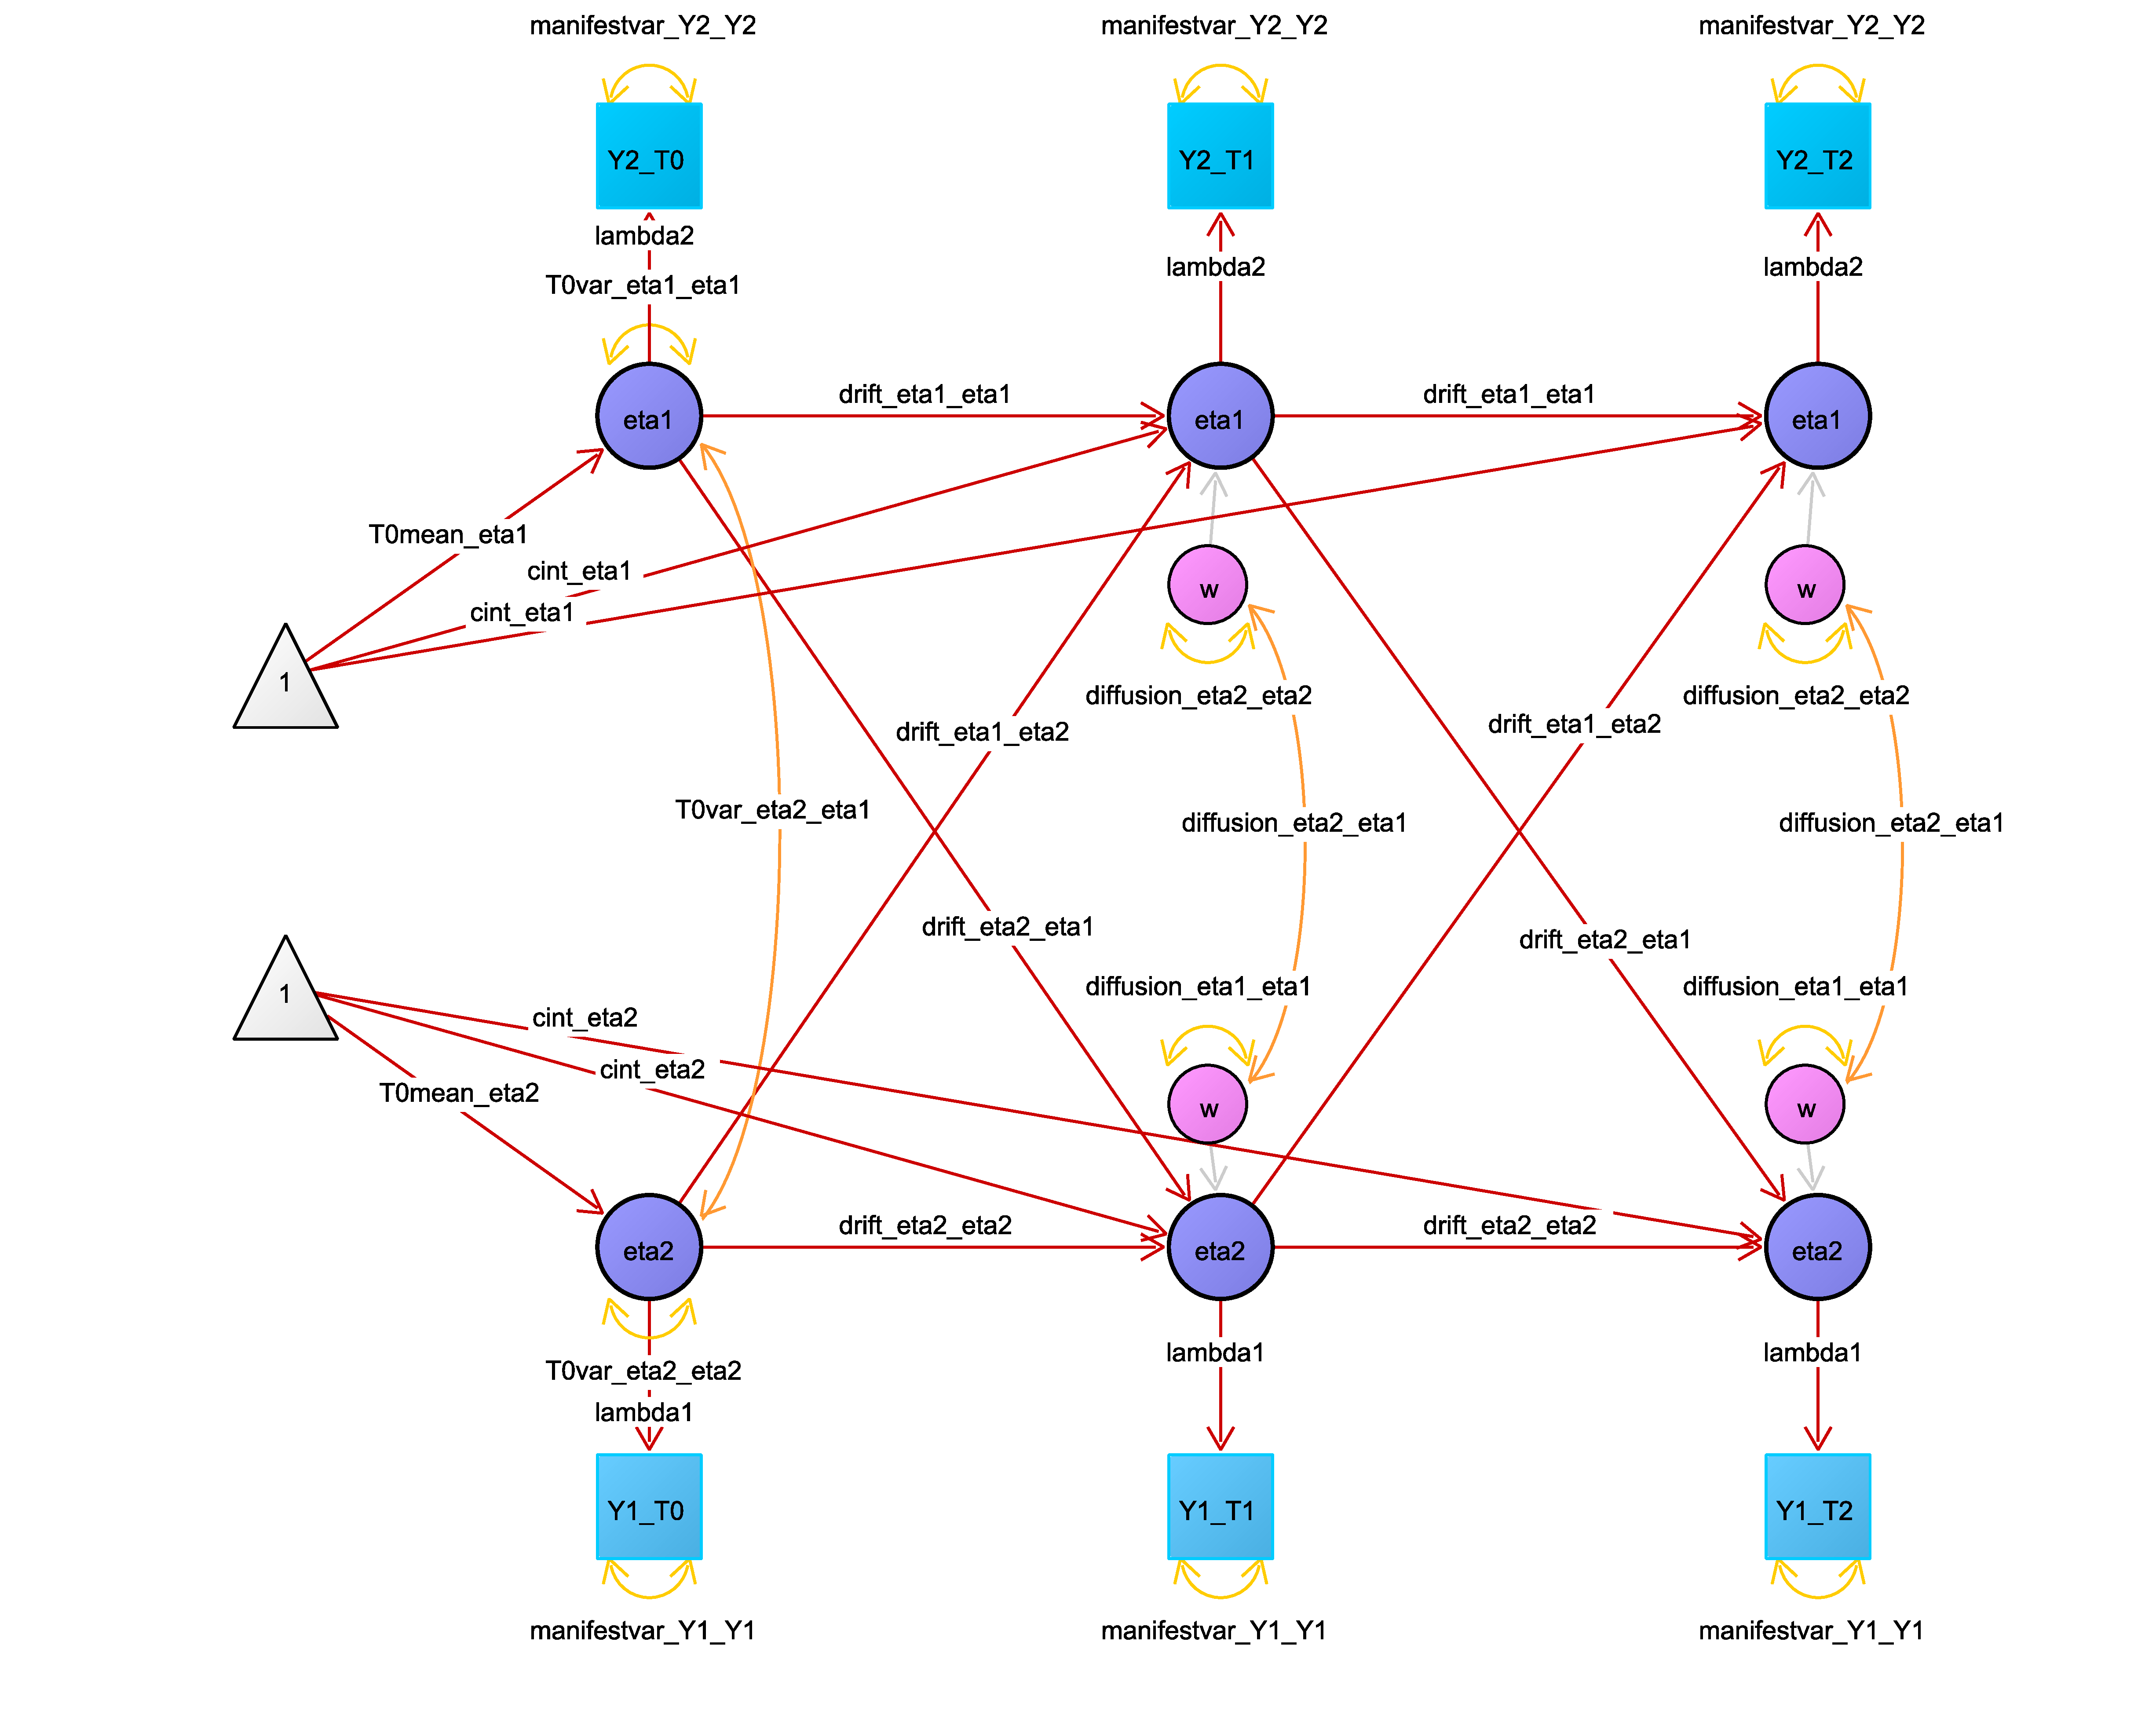
\includegraphics[width = \textwidth]{pathdiagramtwoprocessbasic}
\caption{ \label{fig:pathdiagramtwoprocessbasic} A two process continuous time model with manifest indicators (blue) measuring latent processes (purple). Variance / covariance paths are in orange, regressions in red. Light grey paths indicate those that are either fixed to certain values or constrained to other parameters. Note that the value of the parameters for all paths to latents at time 2 and higher do not directly represent the effect, rather, the effect depends on a function of the shown parameter and the time interval $\Delta$\textit{t}. This model includes neither observed or unobserved between person variance, nor any time dependent predictors. Manifest intercepts are not shown.}
\end{figure}
A visual representation of this model is shown in Figure \ref{fig:pathdiagramtwoprocessbasic}. With \code{n.latent = 2}, we have specified a model with 2 latent processes, shown in purple. Each of these is measured by a single manifest indicator (in blue), for a total of 2 manifest variables, specified with \code{n.manifest = 2}. Loadings between latents and manifests are fixed to 1.00 (indicated by the 2$\times$2 diagonal LAMBDA matrix) at 3 measurement occasions, specified by \code{Tpoints = 3}. Because no other parameters are specified, the model defaults are used, resulting in a bivariate latent process model where each manifest variable has a measurement error variance (manifestvar\_Y1\_Y1, manifestvar\_Y2\_Y2), and a mean fixed to 0. The initial latent variables of each process have freely estimated means (T0mean\_eta1, T0mean\_eta2), variances (T0var\_eta1\_eta1, T0var\_eta2\_eta2), and covariance (T0var\_eta2\_eta1). Subsequent latent variables of each process all have an innovation term, with the variance dependent on a function of the diffusion matrix (variances diffusion\_eta1\_eta1, diffusion\_eta2\_eta2, covariance diffusion\_eta2\_eta1), drift matrix, and time interval $\Delta$\textit{t} (Note that although we speak here of variance and covariance parameters for the sake of intuitive understanding, \pkg{ctsem} works with Cholesky decomposed covariance matrices, discussed in Section \ref{sec:transforms}).
Each latent variable in our two processes has continuous auto effects on itself according to the drift\_eta1\_eta1 and drift\_eta2\_eta2 parameters (the diagonals of the drift matrix), and cross effects to the other process according to the drift\_eta1\_eta2 and drift\_eta2\_eta1 parameters (the off diagonals). This drift matrix combines with time interval $\Delta$\textit{t} to generate the auto and cross regressions shown in the diagram.  As usual, the first process listed in the parameter name represents the row of the drift matrix, and the second the column, with the direction of effects flowing from column to row -- so the parameter drift\_eta1\_eta2 represents the effect of a change in process 2 on later values of process 1. 
Each process also has a continuous intercept (cint{\_}eta1, cint{\_}eta2), which, in combination with the drift matrix, sets the level to which each process asymptotes. These are fixed to zero by default, as the manifest intercepts (via the MANIFESTMEANS matrix) account for non zero levels, by default.
To develop an understanding of the parameter matrices or simply view a model, printing the model object (e.g. \code{print(examplemodel)}) is recommended. To track how these matrices are used within the complete SEM specification, one must first estimate the model (discussed in Section \ref{sec:modelfit}), and may then view the A, S, F or M matrices typical to a RAM specification \citet{mcardle1984algebraic} via \code{example1fit$mxobj$A} (for the A matrix).

\subsubsection{Cholesky decomposed variance / covariance input matrices}\label{sec:transforms}\nopagebreak
To ensure reliable estimation, some parameter transformations have been implemented in \pkg{ctsem} for the estimation of covariance matrices. Rather than directly operate on covariance matrices, \pkg{ctsem} takes as input Cholesky decomposed covariance matrices, as these allow for unbounded estimation. The Cholesky decomposition is such that variance / covariance matrix $\boldsymbol{\Sigma} = LL^\top$, where $L$ is lower-triangular. This means that input variance / covariance matrices for \pkg{ctsem} must be lower triangular. The meaning of a 0 in the matrix is the same for both covariance and Cholesky decomposition approaches. An important point to be aware of is that while Cholesky matrices are required as input, for convenience, the matrices reported in the \code{summary} function are full variance / covariance matrices. These can be converted to the Cholesky decomposed form using code in the form \code{t(chol(summary(ctfitobj)$varcovmatrix))}.

While not affecting interpretations of the matrix input or output, internally, by default \pkg{ctsem} also optimizes over the natural logarithm of the diagonal of the Cholesky factor covariance matrices. These transformations are reflected in the raw \pkg{OpenMx} parameter output section of the output summary (when \code{verbose=TRUE}), but otherwise require no specific knowledge or action -- the logarithmic transformations take place internally, and the regular variance / covariance matrices are displayed in the summary matrices. 

%\subsubsection{Non-singular matrices}\nopagebreak
%To avoid problems with singular matrices, internally, DIFFUSIONlogchol diagonals have .00001 subtracted. This ensures that DIFFUSION diagonals are always positive. When values outside these bounds are input by the user (either as fixed or starting values), the values are adjusted as necessary and the user is informed.

\section{Model estimation} \label{sec:modelfit}\nopagebreak
The \code{ctFit} function estimates the specified model, using the specified data along with the \pkg{ctsem} model object. For an example, we can fit a similar model to that defined in Section \ref{sec:modelspec}. We first load an example dataset contained in the \pkg{ctsem} package, then use the \code{ctFit} function for parameter estimation. Output information can be obtained via the \code{summary} function. The dataset used in this example, is a simulation of the relation between leisure time and happiness for 100 individuals across 6 measurement occasions.  Because our data here does not use the default manifest variable names of \code{Y1} and \code{Y2}, but rather \code{LeisureTime} and \code{Happiness}, we must include a \code{manifestNames} character vector in our model specification.  Because each manifest directly measures a latent process, we can use the same character vector for the \code{latentNames} argument, though one could specify any character vector of length 2 here, or rely on the defaults of \code{eta1} and \code{eta2}. 

\begin{Schunk}
\begin{Sinput}
data("ctExample1")
example1model <- ctModel(n.latent = 2, n.manifest = 2, Tpoints = 6, 
  manifestNames = c("LeisureTime", "Happiness"), 
  latentNames = c("LeisureTime", "Happiness"), LAMBDA = diag(2))
example1fit <- ctFit(dat = ctExample1, ctmodelobj = example1model)
\end{Sinput}
\end{Schunk}

The output of \code{summary} after fitting such a model includes the matrices representing the continuous time parameters (e.g., DRIFT), a list of estimates of only the free parameters, and fit information from the \code{OpenMx} summary function. Further information can be obtained using the argument \code{verbose=TRUE}, which will return the raw \pkg{OpenMx} parameter values and standard errors, as well as additional summary matrices of discrete time transformations for the time interval $\Delta t = 1$ (e.g., discreteDRIFT), and when appropriate, asymptotic values for the parameters as the time interval $\Delta t$ approaches $\infty $ (e.g., asymDIFFUSION may be taken to represent the total within subject variance of a process). When appropriate, standardised matrices are also output with the suffix `std'.\footnote{Standardisations are based on only the relevant variance, not the total. For instance, DRIFT parameters are standardised using only the within-subject variance, asymDIFFUSION, because DRIFT parameters are typically intended to represent individual, or average individual, temporal dynamics.}   

\begin{Schunk}
\begin{Sinput}
summary(example1fit, verbose = TRUE)["discreteDRIFTstd"]
\end{Sinput}
\begin{Soutput}
$discreteDRIFTstd
            LeisureTime Happiness
LeisureTime      0.9728   -0.0499
Happiness       -0.0138    0.9146
\end{Soutput}
\end{Schunk}

The output above shows the standardised discrete time equivalent of the DRIFT matrix for time interval $\Delta t = 1$. This is provided for convenience, but one should note that it only represents the temporal effects given the specific interval of 1 unit of time (The specific interval shown for the discrete summary matrices may be modified with the argument \code{timeInterval}).  The unstandardised discreteDRIFT matrix may be calculated from the continuous drift matrix for any desired interval. The following code shows this calculation for a time interval of 2.5: 

\begin{Schunk}
\begin{Sinput}
expm(summary(example1fit)$DRIFT * 2.5)
\end{Sinput}
\end{Schunk}

See Equation \ref{eq:solution} to understand how this arises. From the diagonals of the discreteDRIFTstd matrix we see that changes in the amount of leisure time one has tend to persist longer (indicated by a higher autoregression) than happiness. The cross-regression in row 2 column 1 suggests that as leisure time increases, this tends to be followed by \textit{decreases} in happiness. Similarly, the cross-regression in row 1 column 2 suggests that as happiness increases, this tends to be followed by \textit{decreases} in leisure time. While these results are accurate for the specified model, the specified model is likely inappropriate for this data, which we explain more of in Section \ref{sec:heterogeneity} on unobserved heterogeneity.

\subsection{Comparing different models} \label{sec:testing}\nopagebreak
Suppose we wanted to test the model we fit above against a model where the effect of happiness on later leisure time (parameter drift\_LeisureTime\_Happiness) was constrained to 0. First we specify and fit the model under the null hypothesis by taking our previous model and fixing the desired parameter to 0:

\begin{Schunk}
\begin{Sinput}
testmodel <- example1model
testmodel$DRIFT[1, 2] <- 0
testfit <- ctFit(dat = ctExample1, ctmodelobj = testmodel)
\end{Sinput}
\end{Schunk}

The result may then be compared to the original model with a likelihood ratio test, using the \pkg{OpenMx} function \code{mxCompare}. To use this function a base model fit object and a comparison model fit object must be specified, with the latter being a constrained version of the former. Note that \pkg{ctsem} stores the original \pkg{OpenMx} fit object under a \code{$mxobj} sub-object, which must be referenced when using \pkg{OpenMx} functions directly.
\begin{Schunk}
\begin{Sinput}
mxCompare(example1fit$mxobj, testfit$mxobj)
\end{Sinput}
\begin{Soutput}
   base comparison ep minus2LL   df  AIC diffLL diffdf          p
1 ctsem       <NA> 16     4177 1184 1809     NA     NA         NA
2 ctsem      ctsem 15     4197 1185 1827   19.9      1 0.00000833
\end{Soutput}
\end{Schunk}
According to the conventional \textit{p} < .05 criterion, results show that the more constrained model fits the data significantly worse, that is, happiness has a significant effect on later leisure time for this model and data. 
An alternative to this approach is to estimate 95\% profile-likelihood confidence intervals for our parameters of interest, from our already fit model:

\begin{Schunk}
\begin{Sinput}
example1cifit <- ctCI(example1fit, confidenceintervals = "DRIFT")
\end{Sinput}
\begin{Soutput}
                               lbound estimate  ubound note
drift_LeisureTime_LeisureTime -0.0468  -0.0280 -0.0125     
drift_LeisureTime_Happiness   -0.1083  -0.0697 -0.0377     
drift_Happiness_LeisureTime   -0.0312  -0.0111  0.0087     
drift_Happiness_Happiness     -0.1486  -0.0896 -0.0459     
\end{Soutput}
\end{Schunk}

Now the \code{summary} function reports 95\% confidence bounds for the continuous drift parameters, which in case of drift\_LeisureTime\_Happiness (DRIFT[1,2]) does not include 0. For complicated models, the estimation of confidence intervals may increase computation time considerably.  One could also compute a confidence interval by multiplying the standard error of the estimate (returned in the summary) by 1.96, however profile-likelihood confidence intervals are in general recommended as they do not assume symmetric intervals, which may be quite unlikely for such models. We have observed however that optimization difficulties can sometimes result in inacccurate (extremely close to the point estimate, accuracy can be checked in the lower and upper delta returned by \code{example1cifit$mxobj$intervals} subobject) or missing profile-likelihood confidence intervals, so the use of standard error based intervals can provide a helpful sanity check. 

\subsection{Plots}\nopagebreak
A visual depiction of the relationships between the processes over time is given by the \code{plot.ctsemFit} (which can be called simply by \code{plot}) function for any fit object created by \code{ctFit}. Depending on arguments, this function can show the processes' mean trajectories, within-subject variance, autoregression, and cross regression plots, as well as plots showing expected changes in each process given either an \textit{observed} change of 1.00, or an \textit{exogenous input} of 1.00 (The former is a mixture of the DIFFUSION and DRIFT matrices, while the latter is just an alternative representation of the auto and cross regression plots). Autoregression plots show the impact of a 1 unit change in a process on later values of that process, while cross regression plots show the impact of a 1 unit change in one process on later values of other processes. Some examples can be seen in Figure \ref{fig:traitparamplots}.

\section{Continuous time models: extensions} \label{sec:extensions}\nopagebreak
\subsection{Unobserved heterogeneity}\nopagebreak
\subsubsection{Traits at the latent level} \label{sec:heterogeneity} \nopagebreak
When modelling panel data, the continuous intercept parameter $\boldsymbol{\kappa}$ reflects the expected value for continuous time intercept $\boldsymbol{\xi}$, which determines the average level of a process ($\boldsymbol{\kappa}$ is fixed to 0 in \pkg{ctsem} by default, as free manifest means account for non zero equilibrium levels in the data). In panel data, however, it is common that \textit{individuals} exhibit stable differences in the level. Within \pkg{ctsem} we call such stable differences \textit{traits}, but they may also be thought of more abstractly as \textit{unit level} or \textit{between subject} differences, or \textit{unobserved heterogeneity}. Fitting a model that fails to account for it will result in parameter estimates that will not reflect the processes of individual subjects, but will mix between and within-person information \citep{balestra1966pooling, oud2000continuous, halaby2004panel}. 
To avoid this bias, individual differences can be incorporated in two different ways. One way is to control for observed covariates as will be discussed in Section \ref{sec:tipreds}. However as covariates are likely to be insufficient, one may also estimate the latent trait variance by estimating the variance and covariance $\boldsymbol{\phi}_{\xi}$ of the intercept parameters $\boldsymbol{\xi}$ across individuals.\footnote{Note that this is a substantially different approach to achieve unbiased effect estimates than the \textit{fixed effects} approach \citep[see for example][]{mundlak1978pooling}, as our SEM specification, while a \textit{random effects} model which have at times been associated with bias for within effects, allows unbiased estimation of \textit{within} and \textit{between} effects at the same time. For further details on the estimation of unobserved heterogeneity in an SEM context, see \citet{bollen2010general}.} In \pkg{ctsem}, freely estimated latent trait variances and covariances may be added with the argument \code{TRAITVAR = "auto"} to the \code{ctModel} command. If the user is interested in a specific variance-covariance structure, it is of course also possible to specify the n.latent $\times$ n.latent lower-triangular matrix of free or fixed parameters by hand. To illustrate the inclusion of trait variance, we fit the same model on simulated leisure time and happiness introduced above, but also model the traits. 

\begin{Schunk}
\begin{Sinput}
data("ctExample1")
traitmodel <- ctModel(n.manifest = 2, n.latent = 2, Tpoints = 6, 
  LAMBDA = diag(2), manifestNames = c("LeisureTime", "Happiness"), 
  latentNames = c("LeisureTime", "Happiness"), TRAITVAR = "auto")
traitfit <- ctFit(dat = ctExample1, ctmodelobj = traitmodel)
\end{Sinput}
\end{Schunk}

\begin{figure}[!h]
\begin{Schunk}


{\centering \includegraphics[width=\maxwidth]{figures/plots-traitparamplot-1} 

}

\end{Schunk}
\caption{ \label{fig:traitparamplots} Top row shows parameter plots without accounting for trait variance, bottom row with trait variance accounted for. Plots show how auto and cross effects change depending on the length of time between observations.}
\end{figure}
From Figure \ref{fig:traitparamplots}, we can see that after accounting for differences in the trait levels of leisure time and happiness, the estimated auto and cross regression effects between latent processes are very different. Auto effects (persistence) have reduced, and the magnitude and sign of the cross effects have switched. Now, rather than a \textit{decrease in leisure time} predicting an \textit{increase in happiness}, after controlling for unobserved heterogeneity we see instead that \textit{increases in leisure time} predict later \textit{increases in happiness}. 

\subsubsection{Traits at the indicator level} \label{sec:manifesttraits}\nopagebreak
Beyond differences in the level of the latent process, it is also possible that stable individual differences in the level of some or all indicators of a process may exist, and as such may be better accounted for at the measurement level. Take for instance a latent process, happiness, estimated using three survey questions at 10 time points for multiple individuals. According to the models we have described so far, the estimated manifest means apply equally to all individuals. However, consider that question three queries happiness with work, which may for some people be consistently high, independent of their actual latent happiness, and for some may be consistently low. Calculating the latent process using the same mean for happiness with work again confounds between and within person information, but we can account for this by using what we will refer to as \textit{manifest traits} -- an additional, time invariant variance-covariance structure on the measurement level. These are specified by including the \code{MANIFESTTRAITVAR} matrix in the \code{ctModel} specification, either as \code{MANIFESTTRAITVAR = "auto"} wherein time invariant variance and covariance for all indicators is freely estimated, or the n.manifest $ \times $ n.manifest lower-triangular matrix can be specified explicitly as usual. Such a specification may allow for improved fit of factor models, more realistic estimates of the dynamics of individual processes, and the testing of measurement related hypotheses. Note however that identifying restrictions will be necessary for any model that contains both manifest and process level traits -- one possible form for this may be a free process level TRAITVAR matrix and a MANIFESTTRAITVAR matrix that is fixed to 0 across factors, but free within any factors that are measured by more than one indicator.
% Further, when combining time dependent predictors (Section \ref{sec:predictors}) in a model with manifest traits, covariance between time dependent predictors and manifest traits will not be accounted for and biased estimates may ensue. 

\subsection{Predictors} \label{sec:predictors}\nopagebreak
\pkg{ctsem} allows the inclusion of \textit{time independent} as well as time \textit{time dependent} exogenous predictors. Time independent predictors could be variables such as gender, personality or socio-demographic background variables that remain constant over time. An example of a time dependent predictor could be a financial crisis, which all individuals in the sample experience at the same time, or the death of a loved one, which only some individuals may experience and for whom the time point of the event may differ. Both events may be thought of as adding some relatively distinct and sudden change to an individual's life, which influences the processes of interest. Time dependent predictors are distinguished from the endogenous latent processes in that they are assumed to be independent of fluctuations in the processes -- changes in the latent processes do not lead to changes in the predictor. Furthermore, no temporal structure between different time points is modeled. Because of these two assumptions, in any case where the time dependent predictor depends on earlier values of either itself or the latent process, it may be better to model it as an additional latent process.

\subsubsection{Time independent predictors} \label{sec:tipreds}\nopagebreak
Time independent predictors are added by including the data as per the structures shown in Section \ref{sec:datastructure}, and specifying the number of time independent predictors, \code{n.TIpred}, in the \code{ctModel} arguments. If not using the default variable naming, a \code{TIpredNames} character vector should also be specified. For an example, we add the `number of close friends' as a time independent predictor to the earlier leisure time and happiness model. Note that, just like in any conventional regression analysis, if time independent predictors are not centered around 0, the estimate of continuous intercept parameters depends on the mean of the predictor. 

\begin{Schunk}
\begin{Sinput}
data("ctExample1TIpred")
tipredmodel <- ctModel(n.manifest = 2, n.latent = 2, n.TIpred = 1,
  manifestNames = c("LeisureTime", "Happiness"),
  latentNames = c("LeisureTime", "Happiness"),
  TIpredNames = "NumFriends",
 Tpoints = 6, LAMBDA = diag(2), TRAITVAR = "auto")
tipredfit <- ctFit(dat = ctExample1TIpred, ctmodelobj = tipredmodel)

summary(tipredfit, verbose = TRUE)["TIPREDEFFECT"]
summary(tipredfit, verbose = TRUE)["discreteTIPREDEFFECT"]
summary(tipredfit, verbose = TRUE)["asymTIPREDEFFECT"]
summary(tipredfit, verbose = TRUE)["addedTIPREDVAR"]
\end{Sinput}
\end{Schunk}
\begin{minipage}[t]{0.5\textwidth}
\begin{Schunk}
\begin{Soutput}
$TIPREDEFFECT
            NumFriends
LeisureTime     -0.226
Happiness        0.549
\end{Soutput}

\begin{Soutput}
$discreteTIPREDEFFECT
            NumFriends
LeisureTime     -0.239
Happiness        0.442
\end{Soutput}
\end{Schunk}
 \end{minipage}
\begin{minipage}[t]{0.5\textwidth}
\begin{Schunk}
\begin{Soutput}
$asymTIPREDEFFECT
            NumFriends
LeisureTime     -1.673
Happiness        0.219
\end{Soutput}

\begin{Soutput}
$addedTIPREDVAR
            LeisureTime Happiness
LeisureTime       2.838   -0.3719
Happiness        -0.372    0.0487
\end{Soutput}
\end{Schunk}
\vspace{\baselineskip}
\end{minipage}

The matrices output from \code{summary, verbose = TRUE} will now include matrices related to time independent predictors, while the estimated parameters now also includes a range of variance, covariance, and effect parameters for time independent predictors.  Matrix TIPREDEFFECT displays the continuous time effect parameters, however discreteTIPREDEFFECT shows the effect added to the processes for each unit of time, which may provide a useful comparison with discrete time models. asymTIPREDEFFECT (Asymptotic time independent predictor effect) shows the expected total change in process means given an increase of 1 on the time independent predictor.  From these matrices we see that the number of close friends has a negative relationship to leisure time, but a positive relationship to happiness. The final matrix, addedTIPREDVAR, displays the stable between-subject variance and covariance in the processes accounted for by the time independent predictors.

\subsubsection{Time dependent predictors} \label{sec:tdpreds}\nopagebreak
\pkg{ctsem} allows the specification of time dependent predictors: The fundamental form of such a predictor is that of a sudden impulse to the system which then dissipates back to the process mean, however with some thought it is possible to specify a wide range of effect shapes. Figure \ref{fig:tdpredtypes} provides an example of two different extremes, the basic impulse form and a permanent level change form.

\begin{figure}[!h]
\begin{Schunk}


{\centering \includegraphics[width=\maxwidth]{figures/plots-tdpreddemo-1} 

}

\end{Schunk}
\caption{ \label{fig:tdpredtypes} Two shapes of time dependent predictors: both plots show 5 selected individuals data, all experiencing a time dependent predictor at time point 5. The model-based expected trajectory of the predictor effect (including autoregression) is also shown as a solid black line. On the left, the processes spike up and then dissipate, reflecting a transient change, or \textit{impulse}. On the right, the processes trend upwards towards a new equilibrium, reflecting a stable change in the \textit{level}.}
\end{figure}

A single time dependent predictor can be incorporated in a \pkg{ctsem} model by adding the argument \code{n.TDpred = 1} to the \code{ctModel} function, as well as a \code{TDpredNames} vector if not using the default variable naming in your data, then fitting as usual. In the following example, we use the same two simulated processes as above and include an intervention that all individuals experience at time 5. For example, let us assume everyone receives a large amount of money and we are interested in the impact of this monetary gift on leisure time and happiness. We expect that some short term increase in both leisure time and happiness may occur, as people may take holidays or enjoy the unexpected boon otherwise, but we also want to check whether the gift we provide may also cause a longer term adjustment in leisure time or happiness. To this end we first fit a model with the basic impulse effect, coded in the data as a 1 when the intervention occurs and a 0 otherwise.\footnote{While this form of dummy coding works well, if there are predictors with no variance and the TDPREDVAR matrix is not specified, \pkg{ctsem} warns the user and fixes TDPREDVAR to a diagonal matrix with small variance.}   

\begin{Schunk}
\begin{Sinput}
data("ctExample2")
tdpredmodel <- ctModel(n.manifest = 2, n.latent = 2, n.TDpred = 1, 
  Tpoints = 8, manifestNames = c("LeisureTime", "Happiness"), 
  TDpredNames = "MoneyInt", latentNames = c("LeisureTime", "Happiness"),
  LAMBDA = diag(2), TRAITVAR = "auto")
tdpredfit <- ctFit(dat = ctExample2, ctmodelobj = tdpredmodel,
  stationary=c('T0VAR','T0TRAITEFFECT'))
summary(tdpredfit, verbose = TRUE)["TDPREDEFFECT"]
\end{Sinput}
\begin{Soutput}
$TDPREDEFFECT
            MoneyInt
LeisureTime    0.286
Happiness      0.708
\end{Soutput}
\end{Schunk}


The matrices reported from \code{summary(tdpredfit, verbose = TRUE)} will now include those related to the time dependent predictor, and the parameters section will include all the additional free parameters estimated, including many variance and covariance related parameters, and the effect parameters TDpred\_LeisureTime\_MoneyInt and TDpred\_Happiness\_MoneyInt.  Looking at the summary matrices, TDPREDEFFECT shows us the initial impact of the predictor on the processes.  From the matrices, we can see that the monetary intervention relates directly to subsequent increases in both leisure time and happiness. Standardised estimates are not provided because we assume no model for the variance of time dependent predictors.

\subsubsection{Adding a level change predictor}\nopagebreak
To test the longer term changes introduced via the monetary intervention, we must model the impact of the predictor via an intermediate latent process: We fix the intercepts (T0MEANS and CINT) and random variance (T0VAR, DIFFUSION, and TRAITVAR) of this additional process to 0; set changes to persist indefinitely via a diagonal DRIFT value very close to 0 (precisely 0 causes computational problems); fix the impact of the predictor on the new process to 1 (to identify the effect); fix the impact of the two original latent processes on the new process to 0 (via the off-diagonals in the third row of DRIFT); and estimate the impact of the additional process on our original two processes of interest (via the off-diagonals in the third column of DRIFT). Alternatively, one could also estimate the time course of predictor effects by freeing the DRIFT diagonal of the additional process. 

\begin{Schunk}
\begin{Sinput}
data("ctExample2")
tdpredlevelmodel <- ctModel(n.manifest = 2, n.latent = 3, 
  n.TDpred = 1, 
  Tpoints = 8, manifestNames = c("LeisureTime", "Happiness"), 
  TDpredNames = "MoneyInt", 
  latentNames = c("LeisureTime", "Happiness", "MoneyIntLatent"),
  LAMBDA = matrix(c(1,0, 0,1, 0,0), ncol = 3), TRAITVAR = "auto")

tdpredlevelmodel$TRAITVAR[3, ] <- 0
tdpredlevelmodel$TRAITVAR[, 3] <- 0
tdpredlevelmodel$DIFFUSION[, 3] <- 0
tdpredlevelmodel$DIFFUSION[3, ] <- 0
tdpredlevelmodel$T0VAR[3, ] <- 0
tdpredlevelmodel$T0VAR[, 3] <- 0
tdpredlevelmodel$CINT[3] <- 0
tdpredlevelmodel$T0MEANS[3] <- 0
tdpredlevelmodel$TDPREDEFFECT[1:3, ] <- c(0,0,1)
tdpredlevelmodel$DRIFT[3, ] <- c(0,0,-.000001)

tdpredlevelfit <- ctFit(dat = ctExample2, 
  ctmodelobj = tdpredlevelmodel, 
  stationary=c('T0VAR','T0TRAITEFFECT'))

summary(tdpredlevelfit, verbose = TRUE)[c("DRIFT","TDPREDEFFECT")]
\end{Sinput}
\begin{Soutput}
$DRIFT
               LeisureTime Happiness MoneyIntLatent
LeisureTime        -0.1421   -0.2180       0.562021
Happiness           0.0848   -0.0167      -0.348001
MoneyIntLatent      0.0000    0.0000      -0.000001

$TDPREDEFFECT
               MoneyInt
LeisureTime           0
Happiness             0
MoneyIntLatent        1
\end{Soutput}
\end{Schunk}

Now, if we look at column 3 of the DRIFT matrix, we see that the monetary intervention process appears to cause long term increases in leisure time, but potentially reductions in happiness. 

\subsection[N = 1 Time series with multiple indicators]{\textit{N} = 1 time series with multiple indicators} \label{sec:timeseries}
In the examples so far, we have dealt with multiple individuals with relatively few measurement occasions, and latent processes have been estimated by a single indicator. However, \pkg{ctsem} may also be used for the analysis of time series data for single subjects observed at many measurement occasions, as well as the estimation of latent factors estimated from multiple indicators. With single-subject data, a Kalman filter implementation is typically far quicker than the matrix arrangement we use for multiple subjects, however \pkg{ctsem} allows either to be used.  To illustrate these features, we perform a dynamic factor analysis on a single individual, with three manifest indicators measured at 100 occasions. Because the model is fitted to a single individual, we cannot freely estimate both the latent variance and mean at the first measurement occasion, but we must fix the $1 \times 1$ \code{T0VAR} matrix to a reasonable value, or implement stationarity constraints as discussed in Section \ref{sec:datatimescale}. The precise fixed value becomes unimportant as the time series length increases \citep{durbin2012time}. Note that in this example the LAMBDA matrix specifies a loading of 1.00 for manifest Y1 (for identification), while loadings for Y2 and Y3 are freely estimated. Note also that although \pkg{ctsem} uses the Kalman filter by default when a single subject is specified, this can be overridden by specifying the \code{objective = "mxRAM"} argument to \code{ctFit}, if one wishes to use the slower RAM implementation. The Kalman filter may also be specified for multiple subjects. In this case, between subject trait or time independent predictor matrices are ignored -- one may need to account for consistent differences between subjects through pre-processing or thoughtful expansion of the state matrices.

\begin{Schunk}
\begin{Sinput}
data("ctExample3")
model <- ctModel(n.latent = 1, n.manifest = 3, Tpoints = 100, 
  LAMBDA = matrix(c(1, "lambda2", "lambda3"), nrow = 3, ncol = 1))
fit <- ctFit(dat = ctExample3, ctmodelobj = model, objective = "Kalman",
  stationary = c("T0VAR"))
\end{Sinput}
\end{Schunk}

\subsection{Multiple group continuous time models}\nopagebreak
In some cases, certain groups or individuals may exhibit different model parameters. We can investigate group or individual level differences by specifying a multiple group model using the \code{ctMultigroupFit} function. For this example, we will use the same model structure as in the single subject example from Section \ref{sec:timeseries}, but apply it to two groups of 10 individuals, whom we expect to exhibit differences in the loading of the third manifest variable. When using \code{ctMultigroupFit}, all parameters are free across groups by default. However, in addition to the standard model specification you may also specify either a \textit{fixed model}, or a \textit{free model}. A fixed model should be of the same structure as the base model, with any parameters you wish to constrain across groups set to the character string `groupfixed'.  The value for any other parameters is not important. Alternatively, one may specify a free model, where any parameters to freely estimate for each group are given the label `groupfree', and all others will be constrained across groups. In this example, because we only want to examine group differences on one parameter, we specify a free model in which the loading parameter between manifest3 and our latent process eta1 is labelled `groupfree' -- this estimates distinct lambda3 parameters for each group, and constrains all other parameters across the two groups to equality. The group specific parameter estimates will appear in the resulting summary prefixed by the specified \textit{grouping vector}. This is the final requirement for \code{ctMultigroupFit} and is simply a vector specifying a group label for each row of our data. In this case we have groups one and two, containing the first and the last 10 rows of data respectively, prefixed by the letter `g' to denote group.

\begin{Schunk}
\begin{Sinput}
data("ctExample4")

basemodel <- ctModel(n.latent = 1, n.manifest = 3, Tpoints = 20,
  LAMBDA = matrix(c(1, "lambda2", "lambda3"), nrow = 3, ncol = 1))

freemodel <- basemodel
freemodel$LAMBDA[3, 1] <- "groupfree"
groups <- paste0("g", rep(1:2, each = 10))

multif <- ctMultigroupFit(dat = ctExample4, groupings = groups,
  ctmodelobj = basemodel, freemodel = freemodel)
\end{Sinput}
\end{Schunk}

\begin{Schunk}
\begin{Soutput}
g1_lambda3 g2_lambda3 
    1.6262     0.0228 
\end{Soutput}
\end{Schunk}

Looking at the estimated parameters from the \code{$omxsummary} (\pkg{OpenMx}) portion of \code{summary, verbose = TRUE}, we indeed see a difference between parameters g1\_lambda3 (group 1) and g2\_lambda3 (group 2), and could test this with the usual approaches discussed in Section \ref{sec:testing}. A point to note is that the multiple group and Kalman filter implementations can be easily combined by specifying a distinct group for each row of data. This can allow for a mixture of individual and group level parameters.

\subsection{Higher order models and simulating data} \label{sec:diffusiondynamics}\nopagebreak
In the models discussed so far, the individual processes were only conceived of as first order processes, always tending to revert to baseline when away from it. However, what about a situation where we have variables which show very slow patterns of change, upwards or downwards trajectories that are maintained over many observations? This can provide for oscillations and slower patterns of change, as for example with damped linear oscillators, or moving average like effects as from the ARMA modelling framework.

%' The difference between a standard autoregressive process and an autoregressive process with autoregression on the diffusion process is depicted in Figure \ref{fig:diffusiondynamics}. 
%' \begin{figure}[!h]
%' <<dynamicresidualplot, cache = FALSE, echo = FALSE, fig.height = 5>>=
%' par(mfrow = c(1, 2), cex = .7)
%' 
%' Tpoints = 60
%' testm <- ctModel(Tpoints = Tpoints, n.latent = 2, n.TDpred = 0, n.TIpred = 0, n.manifest = 2, LAMBDA = diag(1, 2),
%'   DRIFT = matrix(c(-.09, .0, 10, -99), nrow = 2),
%'   DIFFUSION = matrix(c(0, 0, 0, 3.01), 2), CINT = matrix(c(0, 0), nrow = 2), T0MEANS = matrix(0, ncol = 1, nrow = 2),
%'   T0VAR = diag(100, 2))#TRAITVAR = matrix(c(0, .0, .0, .0), nrow = 2, ncol = 2))
%' testd <- ctGenerate(testm, n.subjects = 1, burnin = 100)
%' plot(testd[1, seq(1, 120, 2)], main = 'Autoregressive process', type = "b", col = "red", xlab = "Time", ylab = "Dependent variable")
%' grid()
%' points(testd[1, seq(2, 120, 2)], col = "blue", pch = 2)
%' legend('topleft', legend = c('Process', 'Innovation'), col = c('red', 'blue'), bty = 'n', text.col = c('red', 'blue'), pch = c(1, 2))
%' 
%' testm1 <- ctModel(Tpoints = Tpoints, n.latent = 2, n.TDpred = 0, n.TIpred = 0, n.manifest = 2, LAMBDA = diag(1, 2),
%'   DRIFT = matrix(c(-.22, .0, 1, -.1), nrow = 2),
%'   DIFFUSION = matrix(c(0, 0, 0, .008), 2), CINT = matrix(c(0, 0), nrow = 2), T0MEANS = matrix(0, ncol = 1, nrow = 2),
%'   T0VAR = diag(.05, 2))#, TRAITVAR = matrix(c(0, .0, .0, .0), nrow = 2, ncol = 2))
%' testd1 <- ctGenerate(testm1, n.subjects = 1, burnin = 10)
%' plot(testd1[1, seq(1, 120, 2)], main = 'Autoregressive process with \n autoregressive diffusion', type = "b", col = "red",
%'   xlab = "Time", ylab = "Dependent variable")
%' grid()
%' points(testd1[1, seq(2, 120, 2)], col = "blue", pch = 2)
%' legend('topright', legend = c('Process', 'Innovation'), col = c('red', 'blue'), bty = 'n', text.col = c('red', 'blue'), pch = c(1, 2))
%' @
% \caption{ \label{fig:diffusiondynamics} Difference between a process with only autoregression on the process itself (left) and process with an autoregression on the diffusion also (right) -- note the smooth trends in the right process in comparison to the random direction changes in the left process, as well as some persistence in innovation values generated by the diffusion process (rescaled for ease of comparison).}
% \end{figure}
Continuous time models of this variety are theoretically plausible, as changes to the level of a process are not necessarily always random in direction with a tendency to baseline, but may depend on contextual circumstances that have some persistence.  Consider an individual's overall health over the course of 20 years, sampled every few months.  If the individual changes exercise or eating habits, changes in health do not manifest instantly, rather we could expect either a slow increase or slow reduction, depending on whether the change of habits was positive or negative. Thus, for many measurements, the change in health from the previous measurement will likely be in the same direction as the change was one step earlier. The following details how to specify such a model, generate data using the \code{ctGenerate} function, simply plot the generated data, and estimate the parameters.
% Failing to account for consistency in the diffusion will create misspecification (biased parameter estimates and confidence intervals) in the model. This is similar to the situation with ARMA modelling when the moving average process is not included or misspecified (see \citet{granger1974spurious} for the general ARMA case, and \citet{hamaker2003arma-based} for a treatment using SEM), as the autoregression on the diffusion here achieves a similar result -- past innovations influence future innovations. With \pkg{ctsem}, this autoregressive diffusion can be included (and hence, tested) by endogenising the diffusion process -- treating it as a new latent process without any manifest indicators. To do this for a single process, we specify the model as before, but with an additional latent process and some additional constraints \citep[For more details on this form of specification, see][]{oud2008continuous, delsing2008analyzing}.
% Moving average terms achieve this by incorporating the effect of \textit{l} past innovations. This is however inconsistent with a view of continuously evolving processes through time, as suddenly after \textit{l} observations the effect is gone. Furthermore, if modeled in continuous time, the length of time past innovations would maintain influence would depend on the number of observations in the specific time window -- but why should we assume that the act of observing is altering the impact of past innovations? In contrast to these problems an autoregressive diffusion in continuous time can allow for slower, smoother trends in a manner consistent with a view of processes that evolve continuously -- there is no point reached where suddenly the influence of past innovations drops to 0, rather they decay exponentially with time according to the continuous DRIFT matrix. 

\begin{Schunk}
\begin{Sinput}
genm <- ctModel(Tpoints = 200, n.latent = 2, n.manifest = 1, 
  LAMBDA = matrix(c(1, 0), nrow = 1, ncol = 2),
  DIFFUSION = matrix(c(0, 0, 0, 1), 2),
  MANIFESTVAR = t(chol(diag(.6,1))),
  DRIFT = matrix(c(0, -.1, 1, -.2), nrow = 2),   
  CINT = matrix(c(1, 0), nrow = 2))

data <- ctGenerate(genm, n.subjects = 1, burnin = 200)

ctIndplot(data, n.subjects = 1 , n.manifest = 1, Tpoints = 200)

model <- ctModel(Tpoints = 200, n.latent = 2, n.manifest = 1, 
  LAMBDA = matrix(c(1, 0), nrow = 1, ncol = 2),
  DIFFUSION = matrix(c(0, 0, 0, "diffusion"), 2),
  DRIFT = matrix(c(0, "regulation", 1, "diffusionAR"), nrow = 2))

fit <- ctFit(data, model, stationary = c("T0VAR"))
\end{Sinput}
\end{Schunk}

In the above, we focus on a model for a single subject, and specify with LAMBDA that a single manifest variable measures only the first latent process. With DIFFUSION we specify that only the 2nd unobserved process experiences random innovations. With DRIFT, we specify that the 2nd process has a freely estimated autoregression term, that it directly impacts the first process with a 1:1 relationship, and that as the level of the first process increases, the level of the 2nd process decreases -- providing necessary regulation. 
\subsubsection{Damped linear oscillator}\nopagebreak
\citet{voelkle2013continuous} discuss modelling a damped linear oscillator in detail, however here we demonstrate how to load the data and fit the oscillating model from their paper. In this case, we also specify good starting values with the \code{startValues} argument to \code{ctModel}, and because of this, set the argument \code{carefulFit = FALSE}.

\begin{Schunk}
\begin{Sinput}
data("Oscillating")

inits <- c(-39, -.3, 1.01, 1.01, .1, 1.01, 0.05, .9, 0)
names(inits) <- c("crosseffect","autoeffect", "diffusion",
  "T0var11", "T0var21", "T0var22","m1", "m2", 'manifestmean')

oscillatingm <- ctModel(n.latent = 2, n.manifest = 1, Tpoints = 11,
  MANIFESTVAR = matrix(c(0), nrow = 1, ncol = 1),
  LAMBDA = matrix(c(1, 0), nrow = 1, ncol = 2),
  T0MEANS = matrix(c('m1', 'm2'), nrow = 2, ncol = 1),
  T0VAR = matrix(c("T0var11", "T0var21", 0, "T0var22"), nrow = 2, ncol = 2),
  DRIFT = matrix(c(0, "crosseffect", 1, "autoeffect"), nrow = 2, ncol = 2),
  MANIFESTMEANS = matrix('manifestmean', nrow = 1, ncol = 1),
  DIFFUSION = matrix(c(0, 0, 0, "diffusion"), nrow = 2, ncol = 2),
 startValues=inits)

oscillatingf <- ctFit(Oscillating, oscillatingm, carefulFit = FALSE)
\end{Sinput}
\end{Schunk}

\section[Tips]{Additional specification options and tips for model estimation} \label{sec:tips}\nopagebreak
Given the complexity of parameter constraints, and that for some classes of models multiple minima may exist, parameter estimation is sometimes difficult. To ensure reliable estimation, there are some additional approaches that may be helpful. By default the argument \code{carefulFit = TRUE} for the \code {ctFit} function is specified. This initiates a two-step procedure, in which the first step penalises the likelihood\footnote{The sum of squares of each parameter that is neither factor loading nor mean related is added to the likelihood, as is the inverse of any parameters on the diagonals of square matrices -- essentially penalising values at the extremes} to help maintain potentially problematic parameters close (but not too close!) to 0, and then uses these estimates as starting values for maximum likelihood estimation. Though often useful, in some cases (particularly those with complex dynamics, or user specified starting values) it can help to switch this off. Beyond this, as a general guideline we suggest starting with simpler, more constrained models and freeing parameters in a stepwise fashion (not necessary as a means of model development, simply for fitting purposes). The \code{ctRefineTo} function can be used as a replacement for \code{ctFit} and automates this step-wise progression. One could do this manually by developing the measurement model separately, estimating only autoregressive parameters of the DRIFT matrix at first (in simple models, this means constraining the off-diagonals of the DRIFT matrix to 0), or fixing the factor loading matrix prior to free estimation. For such stepwise progression, the default of small and negative starting values for cross effects should be switched off by argument \code{crossEffectNegStarts = FALSE}, and starting values from the restricted model should be obtained via the \code{omxStartValues} argument, as shown here, using the model fit from from Section \ref{sec:modelfit}:

\begin{Schunk}
\begin{Sinput}
omxInits <- omxGetParameters(example1fit$mxobj)

fitWithInits <- ctFit(dat = ctExample1, ctmodelobj = example1model, 
  omxStartValues = omxInits)
\end{Sinput}
\end{Schunk}

If stepwise model building with starting values based on simpler fits still fails to produce an improved solution, some of the following suggestions may be helpful.
The time scale, although theoretically unimportant in the sense that all time ranges can be accounted for, can be computationally relevant. It is helpful to choose a scale that roughly matches the expected dynamics -- for instance a time scale of nanoseconds for panel data measured yearly would be problematic, instead, a yearly or monthly time scale could be used. 
Centering the \textit{grand} mean of the variables to 0 may help, as can standardising the variances, particularly in cases where both a measurement model and dynamic model are estimated. 
% Standard errors are reported based on the calculated hessian in OpenMx \citep{boker2011openmx:}, as these may not be optimal in some situations maximum likelihood confidence intervals on any parameters may be calculated via the \code{confidenceintervals} argument to \code{ctFit}. This simply passes the request through to OpenMx. Additionally, we have observed that in some circumstances estimating confidence intervals can lead the optimizer to an improved and more consistent point estimate.
% In some circumstances, optimization difficulty may be due to the highly non-linear nature of changes in the parameters -- a change of .01 to the drift11 parameter makes a much larger difference when drift11 is near 0 than when it is -100. This difficulty can be alleviated by setting the \code{discreteOptimize = TRUE} argument to \code{ctFit}, which rearranges the various algebraic constraints within the model so that discrete equivalent (for $\Delta t = 1$) parameters are optimised over instead. These parameters will be reported in the summary, which may also make interpretation easier. In our experience so far this approach works consistently, but some care should be taken in interpretation as matrix logarithm functions (necessary for this approach) are not defined in all circumstances -- an inverted autoregressive relationship is one possibility, though should at least be quite obvious. 
One way to search for an improved solution is simply to try many times with varying starting values. This is automated by default using the \code{mxTryHard} function from \pkg{OpenMx}, however you may want to increase the \code{retryattempts} argument to \code{ctFit}, or simply re-run \code{ctFit} many times, as it generates unspecified starting values with some limited randomness.  However, since both automated procedures begin within a similar range, for truly problematic cases one may consider adding more extensive randomness to the starting values manually.
In situations with a limited number of time points or of high complexity, you may implement the stationarity assumption, so that parameters related to the first time point are no longer estimated, but constrained to the asymptotic effects, when the time interval $\Delta t\to\infty$. This can make optimization more straightforward, and may serve as a useful basis for determining starting values, or as a viable model in itself.  For more discussion regarding stationarity conditions see Section \ref{sec:datatimescale}. 
In some cases, optimizing over the continuous time parameters (the default) results in fits that do not pass every check and you may be left with warnings. If this occurs, you can instead optimize over asymptotic variants of the parameters, by using the argument \code{asymptotes = TRUE} to \code{ctFit}. This will in general produce equivalent results if the DIFFUSION, CINT, and TIPRED matrices are all freely estimated, even though the raw parameters of these matrices will look different. If these matrices have been constrained in some way, this approach is not recommended.

\subsection{Optimization performance}\nopagebreak
When time intervals vary for every individual, optimization can be quite slow.  To quickly estimate approximate versions of a model, you may use the \code{meanIntervals = TRUE} argument to \code{ctFit}, which will set every individual's time intervals to the mean of the interval across all individuals. A step further even is to specify the argument \code{objective = "cov"} in order to estimate a covariance matrix from the supplied data and fit directly to that. In cases with variability in time intervals these approaches will substantially speed up optimization, but also waste information and bias parameters. Using such an approach in combination with a constrained DRIFT matrix to generate starting values may be a reasonable way to improve fitting speed and generate starting values for large and complex models.

\section[Limitations and future directions]{Limitations and future directions} \label{sec:limitations}\nopagebreak
Currently, a number of assumptions are present in the specification of continuous time models implemented in \pkg{ctsem}. Although the processes are allowed to begin at different levels and variances, from then on a time-invariant model is assumed. Thus, \pkg{ctsem} cannot presently account for time-varying aspects of the processes, except in the form of observed exogenous inputs via time dependent predictors. Although as with many discrete models we could free various parameters across measurement occasions, their meaning would become unclear, as each measurement occasion (set of n.manifest columns in the wide format data) may contain observations from many different times. Instead, models which allow parameters to vary as a function of time could be incorporated in the future as per the time-varying specification in \citet{oud2000continuous}.
As we fit using full information maximum likelihood, standard assumptions regarding multivariate normality apply to manifest variables. Generalisations of the measurement model to allow for non-normal indicators could be implemented using the regular \pkg{OpenMx} functionality however.
% The multi-group implementation has no regularisation applied to the estimation of parameters that are free across groups, hence variance of such parameters may be too large \citep[for a discussion of fixed and random effect models see][]{robinson1991that}. 
% Due to the wide format implementation, expected covariance matrices increase exponentially in size with increases in time points, resulting in slow performance for longer time series. Future versions of \pkg{ctsem} will incorporate the new Kalman filter implementation of \pkg{OpenMx} \citep{neale2015openmx} to alleviate this concern. 
% Exogenous predictors (both time dependent and independent) cannot currently be specified with a measurement model, thus are assumed to be measured without error. This is straightforward to implement (though will involve more assumptions than present), and may be included at some stage. 
Although we allow for heterogeneity in the level of the processes across individuals, heterogeneity in other parameters is not accounted for, and can only be examined via multiple group approaches.
Presently, effects are assumed to be transmitted near instantaneously, as we do not estimate a dead time between inputs and the effect of inputs. We believe this is unlikely to severely impact estimates unless the dead time is of a similar or greater order of magnitude as the time course of effects, however such a parameter could potentially be incorporated within the continuous time equations \citep{richard2003timedelay}.
Although in such areas \pkg{ctsem} may benefit from expansion, \pkg{ctsem} as it stands allows for the straightforward specification of continuous time dynamic models for both panel and time series data, which may include a measurement model, exogenous predictors, multiple processes, unobserved heterogeneity, multiple groups, as well as easy to specify parameter constraints and more complex dynamic specifications. 
% \section[conclusion]{Summary and Conclusions}
% We have introduced \pkg{ctsem}, an \proglang{R} package for continuous time modelling of panel (\textit{N} > 1) and time series (\textit{N} = 1) data, using structural equation models (SEM). At present, \pkg{ctsem} allows for relatively simple specification and estimation of models containing multiple latent processes measured by multiple noisy indicators with variable measurement occasions within and between individuals. Models with individual differences in base levels of indicators or processes may be estimated, as well as the processes' relation to stable (time indepdendent) and time dependent exogenous predictors. We've shown how these models can be easily specified in a multiple group context also, as well as how one may specify more complex patterns of temporal dependency in the change process. While particularly important as a means of making continuous time modelling more generally accessible, hopefully alleviating the difficulties associated with irregularly gathered data, we also hope to have shown that \pkg{ctsem} incorporates much functionality relevant to longitudinal analysis in general. 
% \label{sec:conclusion}

\section[Acknowledgements]{Acknowledgements}\nopagebreak
We would like to thank the Intra Person Dynamics and the Formal Methods research groups at the Max Planck Institute for Human Development for assistance with this work, as well as Joshua Pritikin and the \pkg{OpenMx} development team for feedback and fast response to issues. The \pkg{Knitr} \citep{xie2015Dynamic} and \pkg{Onyx} \citep{vonoertzen2015structural} software were invaluable in constructing this document.
%% Note: If there is markup in $sub)section, then it has to be escape as above.
\bibliography{ctsemrefs}

\newpage
\appendix
\section{Comparison to discrete time approach}\label{appendix:discretecomparison}\nopagebreak
To highlight the problems associated with treating all time intervals in a dataset as equivalent, in this example we use the data and model specified in Section \ref{sec:heterogeneity}, but set all the time intervals to the mean time interval. 

\begin{Schunk}
\begin{Sinput}
data("ctExample1")
traitmodel <- ctModel(n.manifest = 2, n.latent = 2, Tpoints = 6, 
  LAMBDA = diag(2), manifestNames = c("LeisureTime", "Happiness"), 
  latentNames = c("LeisureTime", "Happiness"), TRAITVAR = "auto")
traitfit <- ctFit(dat = ctExample1, ctmodelobj = traitmodel)
traitfit <- ctCI(traitfit, confidenceintervals = 'DRIFT')

discrete <- ctExample1
discrete[ , paste0('dT', 1:5)] <- mean(discrete[ , paste0('dT', 1:5)])
discretefit <- ctFit(discrete, traitmodel)
discretefit <- ctCI(discretefit, confidenceintervals = 'DRIFT')

summary(traitfit)$omxsummary$Minus2LogLikelihood
\end{Sinput}
\begin{Soutput}
[1] 4151
\end{Soutput}
\begin{Sinput}
summary(traitfit)$omxsummary$CI
\end{Sinput}
\begin{Soutput}
                              lbound estimate ubound note
drift_LeisureTime_LeisureTime -0.535   -0.110  0.227     
drift_LeisureTime_Happiness   -0.362   -0.134  0.182     
drift_Happiness_LeisureTime    0.156    0.387  0.910     
drift_Happiness_Happiness     -0.698   -0.344 -0.173     
\end{Soutput}
\begin{Sinput}
summary(discretefit)$omxsummary$Minus2LogLikelihood
\end{Sinput}
\begin{Soutput}
[1] 4203
\end{Soutput}
\begin{Sinput}
summary(discretefit)$omxsummary$CI
\end{Sinput}
\begin{Soutput}
                              lbound estimate ubound note
drift_LeisureTime_LeisureTime  0.145    0.332     NA  !!!
drift_LeisureTime_Happiness       NA   -0.300 -0.120  !!!
drift_Happiness_LeisureTime    0.229    0.951     NA  !!!
drift_Happiness_Happiness         NA   -0.742 -0.121  !!!
\end{Soutput}
\end{Schunk}

In this case, the log likelihood of the fit is worse, parameter estimates do not look very sensible, and there can be difficulties estimating confidence intervals for some parameters.

\newpage
\section{Package comparisons} \label{app:appendixA}\nopagebreak
The following script loops over a sequence in which data is generated from a very simple model (to facilitate comparison), then various packages are used to fit the data, and the distribution of parameter estimates is then plotted. \pkg{ctsem} is used to generate 500 time points of data for a single individual, for a single perfectly measured, stationary process with a drift value of -0.3. The different packages at times use different transformations of the parameters, but for ease of comparison these are transformed to the drift parameter in \pkg{ctsem}. This comparison is not intended as a critique of any package, differences in intended use and estimation routines may result in the observed differences, and it is hoped the provided code  may help others to explore alternatives when necessary.

\begin{Schunk}
\begin{Sinput}
   if (!requireNamespace("cts", quietly = TRUE)) {
    stop("cts package needed for this function to work. Please install it.",
      call. = FALSE)
  }
  if (!requireNamespace("yuima", quietly = TRUE)) {
    stop("yuima package needed for this function to work. Please install it.",
      call. = FALSE)
  }
Tpoints<-500
output <- matrix(NA, 100, 6)
colnames(output) <- c('True', 'ctsem', 'cts', 'yuima', 'arima', 'OpenMx')
for(i in 1:nrow(output)){
generatingModel <- ctModel(n.latent = 1, n.manifest = 1, 
  Tpoints = Tpoints,
  LAMBDA = diag(1), DRIFT = matrix(-.3, nrow = 1),
  CINT = matrix(3, 1, 1),
  MANIFESTVAR = diag(0.00001, 1),
  DIFFUSION = t(chol(diag(5, 1))))

output[i, 1] <- generatingModel$DRIFT #true value

ctsemData <- ctGenerate(generatingModel, n.subjects=1, burnin=30)
longData <- ctWideToLong(ctsemData, Tpoints=500, n.manifest=1)
longData <- ctDeintervalise(longData)

### ctsem package
ctsemModel <- ctModel(n.latent=1, n.manifest = 1, 
  Tpoints = Tpoints,
  MANIFESTVAR = diag(0.0001, 1),
  LAMBDA = diag(1))
ctsemFit <- ctFit(ctsemData, ctsemModel, stationary = c('T0VAR'))
output[i,2] <- mxEval(DRIFT, ctsemFit$mxobj)

### CTS package
ctsData <- longData[, c('time', 'Y1')]
library(cts)
ctsFit <- car(ctsData, order = 1, scale = 1)
output[i, 3] <- -1 * (1 + ctsFit$phi) / (1 - ctsFit$phi) 

### yuima package (not plotted - potential issues due to dT=1)
library(yuima)
mod <- setModel(drift="drift * x + cint", diffusion = "diffusion")
ou <- setYuima(model = mod, data = setData(longData[,'Y1'], delta = 1))
mlout <- qmle(ou,start = list(drift = -.3, diffusion = 1, cint = 1))
output[i, 4] <- mlout@coef[2]

### arima (from stats package, discrete time analysis only)
arfit <- arima(longData[, 'Y1'], order = c(1, 0, 0))
log(arfit$coef[1]) #transform ar1 parameter to drift parameter
output[i, 5]<-log(arfit$coef[1])

### OpenMx state space function
ctsemModel <- ctModel(n.latent=1, n.manifest = 1, 
  Tpoints = Tpoints,
  MANIFESTVAR = diag(0.0001, 1), T0VAR=diag(1), LAMBDA = diag(1))
cdim <- list('Y1', c('eta1'))

amat <- mxMatrix('Full', 1, 1, TRUE, .3,
	name='A', lbound=-10)
bmat <- mxMatrix('Full', 1, 1, FALSE, 0, name='B')
cmat <- mxMatrix('Full', 1, 1, FALSE, 1, name='C', dimnames=cdim)
dmat <- mxMatrix('Full', 1, 1, TRUE, 1, name='D')
qmat <- mxMatrix('Full', 1, 1, TRUE, 1, name='Q')
rmat <- mxMatrix('Diag', 1, 1, FALSE, .0001, name='R')
xmat <- mxMatrix('Full', 1, 1, TRUE, 7, name='x0', lbound=-10, ubound=10)
pmat <- mxMatrix('Diag', 1, 1, FALSE, 1, name='P0')
umat <- mxMatrix('Full', 1, 1, FALSE, 1, name='u')
tmat <- mxMatrix('Full', 1, 1, name='time', labels='data.time')

osc <- mxModel("AR1", 
	amat, bmat, cmat, dmat, qmat, rmat, xmat, pmat, umat, tmat,
	mxExpectationStateSpace('A', 'B', 'C', 'D', 'Q', 'R', 'x0', 'P0', 'u'),
	mxFitFunctionML(),
	mxData(longData, 'raw'))

oscr <- mxRun(osc)

output[i,6] <-  log(mxEval(A, oscr))

} #end for loop

### plot output
plot(density(output[1:i, 2]), xlim = c(-.4, -.1), lty = 2, lwd = 2, 
  ylab='Density',
  main = 'Density of estimates of drift parameter (true value -0.3)')
points(density(output[1:i, 3]), col='red', type='l', lty=3, lwd=3)
points(density(output[1:i, 5]), col='blue', type='l', lwd=2, lty=2)
points(density(output[1:i, 6]), col='green', type='l', lwd=4, lty=5)
legend('topleft', bty='n', 
  text.col = c('black','red','blue', 'green'),
  legend = c('ctsem', 'cts', 'arima', 'OpenMx'))
\end{Sinput}
\end{Schunk}

\end{document}





